\subsection{COMPOSITION OPERATORS ON AN ALGEBRA OF POLYNOMIALS}

Let K be a commutative field of characteristic 0, and K{[}X{]} the algebra of polynomials in one indeterminate over K (Alg., IV. 1); throughout this section by an operator on K{[}X{]} we shall mean a linear map U of the vector space K{[}X{]} (over K) into itself; since the monomials \(X^{n}\) ( \(n \geqslant 0\) ) form a basis for this space, U is determined by the polynomials \(U(X^{n})\) ; specifically, if \(f(X) = \sum_{k=0}^{\infty} \lambda_{k} X^{k}\) with \(\lambda_{k} \in K\) , then \(U(f) = \sum_{k=0}^{\infty} \lambda_{k} U(X^{k})\) .

If \(\mathbf{G}\) is a commutative algebra over \(\mathbf{K}\) , with an identity element, the \(\mathbf{G}\) -module \(\mathrm{G}[\mathrm{X}]\) is obtained by extending the field of scalars \(\mathbf{K}\) of the vector space \(\mathrm{K}[\mathrm{X}]\) to \(\mathrm{G}\) ; every operator \(U\) on \(\mathrm{K}[\mathrm{X}]\) extends in a unique manner to a linear map of the \(\mathrm{G}\) -module \(\mathrm{G}[\mathrm{X}]\) to itself, which we again denote by \(U\) (Alg., II, p.~278); for each element \(g(\mathrm{X}) = \sum_{k=0}^{\infty} \gamma_k X^k\) , with \(\gamma_k \in \mathrm{G}\) , one has \(U(g) = \sum_{k=0}^{\infty} \gamma_k U(X^k)\) .

Consider in particular the case where \(\mathrm{G} = \mathrm{K}[\mathrm{Y}]\) ; then \(\mathrm{G}[\mathrm{X}]\) is the ring \(\mathrm{K}[\mathrm{X},\mathrm{Y}]\) of polynomials in two indeterminates over \(\mathrm{K}\) ; to avoid confusion we denote the extension of \(U\) to \(\mathrm{G}[\mathrm{X}]\) by \(U_{\mathrm{X}}\) . For any polynomial \(g(\mathrm{X},\mathrm{Y}) = \sum_{k=0}^{\infty}\gamma_k(\mathrm{Y})\mathrm{X}^k\) where \(\gamma_k(Y)\in \mathrm{K}[\mathrm{Y}]\) one thus has \(U_{\mathrm{X}}(g) = \sum_{k=0}^{\infty}\gamma_k(\mathrm{Y})U(\mathrm{X}^k)\) . Since \(U_{\mathrm{X}}\) is linear one sees that if one writes \(g(\mathrm{X},\mathrm{Y}) = \sum_{h=0}^{\infty}\beta_h(\mathrm{X})\mathrm{Y}^h\) then one also has \(U_{\mathrm{X}}(g) = \sum_{h=0}^{\infty}U(\beta_h)\mathrm{Y}^h\) .

Under the canonical isomorphism of K{[}X{]} onto K{[}Y{]} which associates Y with X the operator U transforms to an operator on K{[}Y{]}, which we will denote \(U_{Y}\) , to avoid confusion, so that \(U_{\mathrm{Y}}(f(\mathrm{Y}))\) is the polynomial obtained by replacing X by Y in the polynomial \(U(f(\mathrm{X})) = U_{\mathrm{X}}(f(\mathrm{X}))\) . This operator \(U_{Y}\) can in turn be extended to an operator (again denoted by \(U_{Y}\) ) on K{[}X,Y{]}: if \(g(\mathrm{X}, \mathrm{Y}) = \sum_{h=0}^{\infty} \beta_{h}(\mathrm{X}) \mathrm{Y}^{h}\) then \(U_{\mathrm{Y}}(g(\mathrm{X}, \mathrm{Y})) = \sum_{h=0}^{\infty} \beta_{h}(\mathrm{X}) U_{\mathrm{Y}}(\mathrm{Y}^{h})\) .

As an example of these extensions we cite the derivation operator D on K{[}X{]} (Alg., IV. 6), which gives the partial derivation operators \(D_{X}\) and \(D_{Y}\) on K{[}X,Y{]}.

For any polynomial \(f \in K[X]\) we denote by \(T_{Y}(f)\) the polynomial \(f(X + Y)\) in K{[}X,Y{]}; the map \(T_{Y}\) is a K-linear map from K{[}X{]} into K{[}X,Y{]}, called a translation operator.

DEFINITION 1. One says that an operator U on K{[}X{]} is a composition operator if it commutes with the translation operator, that is, if \(U_{X}T_{Y} = T_{Y}U\) .

In other words, if \(f\) is an arbitrary polynomial in \(\mathbf{K}[\mathbf{X}]\) , and if \(g = U(f)\) , one must have \(g(\mathbf{X} + \mathbf{Y}) = U_{\mathbf{X}}(f(\mathbf{X} + \mathbf{Y}))\) .

It follows immediately from this definition that for every polynomial \(f(\mathrm{X}) \in \mathrm{K}[\mathrm{X}]\) one has, in the above notation,

\[
U _ {\mathrm{X}} \big (f (\mathrm{X} + \mathrm{Y}) \big) = U _ {\mathrm{Y}} \big (f (\mathrm{X} + \mathrm{Y}) \big).\tag{1}
\]

Examples. 1) For every \(\lambda \in \mathbf{K}\) the operator which to every polynomial \(f(\mathbf{X})\) associates the polynomial \(f(\mathbf{X} + \lambda)\) is a composition operator.

\begin{enumerate}
\def\labelenumi{\arabic{enumi})}
\setcounter{enumi}{1}
\tightlist
\item
  The derivation D on K{[}X{]} is a composition operator (cf.~prop. 1).
\end{enumerate}

Remark. Since K is an infinite field the operator U on K{[}X{]} is a composition operator if and only if for every polynomial \(f \in K[X]\) and every element \(\alpha \in K\) one has, putting \(g = U(f)\) , that \(g(X + \alpha) = U(f(X + \alpha))\) . (Alg., IV. 16, cor.).

It is clear that every linear combination of composition operators, with coefficients in K, is a composition operator; the same is true for the composition of two composition operators. In other words, the composition operators form a subalgebra \(\Gamma\) of the algebra of endomorphisms of the vector space K{[}X{]}.

PROPOSITION 1. For an operator U on K{[}X{]} to be a composition operator it is necessary and sufficient that it commute with the derivation D on K{[}X{]}.

Indeed, the Taylor formula shows that for every polynomial \(f \in K[X]\) one has

\[
U _ {\mathrm{X}} \big (f (\mathrm{X} + \mathrm{Y}) \big) = U _ {\mathrm{X}} \left(\sum_ {k = 0} ^ {\infty} \frac {1}{k !} \mathrm{Y} ^ {k} \mathrm{D} ^ {k} f (\mathrm{X})\right) = \sum_ {k = 0} ^ {\infty} \frac {1}{k !} \mathrm{Y} ^ {k} U \big (\mathrm{D} ^ {k} f (\mathrm{X}) \big);
\]

if one puts \(g = U(f)\) then one has

\[
g (\mathrm{X} + \mathrm{Y}) = \sum_ {k = 0} ^ {\infty} \frac {1}{k !} \mathrm{Y} ^ {k} \mathrm{D} ^ {k} g (\mathrm{X}) = \sum_ {k = 0} ^ {\infty} \frac {1}{k !} \mathrm{Y} ^ {k} \mathrm{D} ^ {k} (U (f (\mathrm{X})))
\]

for U to be a composition operator, one must then have \(UD^{k} = D^{k}U\) for every integer \(k \geqslant 1\) , and in particular \(UD = DU\) . Conversely, if this relation holds, it implies \(UD^{k} = D^{k}U\) for every integer \(k \geqslant 1\) , by induction on k; the Taylor formula then shows that \(g(X + Y) = U_{X}(f(X + Y))\) .

For every polynomial \(f \in K[X, Y]\) we denote by \(U_{0}(f)\) the term independent of X in the polynomial \(U_{X}(f)\) ; in particular, if \(f \in K[X]\) , \(U_{0}(f)\) is the constant term in \(U(f)\) , and \(U_{0}\) is a linear form on K{[}X{]}. For every polynomial \(f \in K[X]\) let \(g = U(f)\) ; by def. 1 of VI, p.~270

\[
g (\mathrm{X} + \mathrm{Y}) = U _ {\mathrm{X}} (f (\mathrm{X} + \mathrm{Y})) = U _ {\mathrm{X}} \left(\sum_ {k = 0} ^ {\infty} \frac {1}{k !} \mathrm{X} ^ {k} \mathrm{D} ^ {k} f (\mathrm{Y})\right) = \sum_ {k = 0} ^ {\infty} \frac {1}{k !} U (\mathrm{X} ^ {k}) \mathrm{D} ^ {k} f (\mathrm{Y})
\]

and if, in this formula, one replaces X by 0, one obtains

\[
g (\mathrm{Y}) = \sum_ {k = 0} ^ {\infty} \frac {1}{k !} U _ {0} (\mathrm{X} ^ {k}) \mathrm{D} ^ {k} f (\mathrm{Y}).
\]

Thus one sees that

\[
U (f (\mathrm{X})) = \sum_ {k = 0} ^ {\infty} \frac {1}{k !} \mu_ {k} \mathrm{D} ^ {k} f (\mathrm{X})\tag{2}
\]

where \(\mu_{k}\) is the constant term in the polynomial \(U(\mathbf{X}^k)\) .

This formula shows that the \(\mu_{k}\) determine the composition operator U completely; conversely, if \((\mu_{n})\) is an arbitrary sequence of elements of K then the formula (2) defines an operator U which clearly commutes with D, so (VI, p.~270, prop. 1) is a composition operator. From now on we shall write (2) in the form

\[
U = \sum_ {k = 0} ^ {\infty} \frac {1}{k !} \mu_ {k} D ^ {k}.\tag{3}
\]

This formula can be interpreted in topological language as follows: if one considers the discrete topology on K{[}X{]}, and the topology of simple convergence on the algebra \(\operatorname{End}(\operatorname{K}[X])\) of endomorphisms of K{[}X{]} (Gen.~Top., X, p.~277), the series with general term \(\frac{1}{k!}\mu_{k}D^{k}\) is commutatively convergent in \(\operatorname{End}(\operatorname{K}[X])\) and has sum U (Gen.~Top., III, p.~269).

The formula (3) shows that to every formal series \(u(S) = \sum_{k=0}^{\infty} \alpha_k S^k\) in one indeterminate over \(K\) (Alg., IV. 41) one can associate the composition operator \(U = \sum_{k=0}^{\infty} \alpha_k D^k\) , which in future we shall denote by \(u(D)\) . This remark can be clarified in the following manner:

THEOREM 1. The map which to every formal series \(u(\mathbf{S}) = \sum_{k=0}^{\infty} \alpha_k \mathbf{S}^k\) in one indeterminate over \(\mathbf{K}\) associates the composition operator \(u(\mathbf{D}) = \sum_{k=0}^{\infty} \alpha_k \mathbf{D}^k\) on \(\mathrm{K}[\mathrm{X}]\) is an isomorphism of the algebra \(\mathrm{K}[[\mathrm{S}]]\) of formal series onto the algebra \(\Gamma\) of composition operators.

One verifies immediately that this map is an homomorphism. It remains to see that it is injective, in other words, that the relation \(\sum_{k=0}^{\infty}\alpha_{k}D^{k}=0\) implies \(\alpha_{k}=0\) for every k; now \(h!\alpha_{h}\) is the constant term in the polynomial obtained by applying \(\sum_{k=0}^{\infty}\alpha_{k}D^{k}\) to \(X^{h}\) , whence the theorem.

COROLLARY. The algebra \(\Gamma\) of composition operators in K{[}X{]} is commutative.

Example. If \(U\) is the operator which to each polynomial \(f(\mathrm{X})\) associates \(f(\mathrm{X} + \lambda)\) (where \(\lambda \in \mathbf{K}\) ), one has \(U_0(\mathrm{X}^k) = \lambda^k\) , and so \(U = \sum_{k=0}^{\infty} \frac{1}{k!} (\lambda \mathrm{D})^k\) . By analogy with the series expansion of \(e^x\) (III, p.~105) we write \(e^{\mathrm{S}}\) or \(\exp(\mathrm{S})\) for the formal series \(\sum_{n=0}^{\infty} \frac{1}{n!} \mathrm{S}^n\) in the ring \(\mathrm{K}[[\mathrm{S}]]\) ; so one can write \(U = e^{\lambda \mathrm{D}}\) . Replacing the field \(\mathrm{K}\) by the field of rational fractions \(\mathrm{K}(\mathrm{Y})\) in this argument one sees similarly that the translation operator \(T_{\mathrm{Y}}\) can be written \(e^{\mathrm{YD}}\) .

Furthermore, in the ring K{[}{[}S, T{]}{]} of formal series in two indeterminates over K one has

\[
\begin{array}{l} (\exp S) (\exp T) = \sum_ {p, q} \frac {S ^ {p}}{p !} \frac {T ^ {q}}{q !} \\ = \sum_ {n = 0} ^ {\infty} \frac {1}{n !} \left(\binom {n} {0} S ^ {n} + \binom {n} {1} S ^ {n - 1} T + \dots + \binom {n} {n} T ^ {n}\right) \\ = \exp (S + T) \end{array}\tag{4}
\]

and in particular

\[
(\exp S) (\exp (- S)) = 1\tag{5}
\]

which justifies the notation we have introduced.

Scholium. The isomorphism of the algebra K{[}{[}S{]}{]} of formal series and the algebra \(\Gamma\) of composition operators on K{[}X{]} sometimes allows one to prove propositions on formal series most simply, by proving them for the corresponding composition operators (cf.~VI, p.~274, prop. 6).

\subsection{APPELL POLYNOMIALS ATTACHED TO A COMPOSITION OPERATOR}

Given a composition operator \(U = \sum_{k=0}^{\infty} \alpha_k \mathrm{D}^k \neq 0\) let \(p\) be the least of the integers \(k\) such that \(\alpha_k \neq 0\) ; we shall say that \(p\) is the order of the operator \(U\) .

PROPOSITION 2. Every composition operator of order 0 is invertible in the algebra \(\Gamma\) of composition operators on K{[}X{]}.

Indeed, a formal series \(\sum_{k=0}^{\infty}\alpha_{k}S^{k}\) such that \(\alpha_{0}\neq0\) is invertible in the ring K{[}{[}S{]}{]} (Alg., IV. 41); the proposition thus follows from th. 1 of VI, p.~271.

PROPOSITION 3. Let U be a composition operator of order p; then \(U(f) = 0\) for every polynomial f of degree \textless{} p; for every polynomial \(f \neq 0\) of degree \(n \geqslant p\) , \(U(f)\) is a polynomial \(\neq 0\) of degree n - p.

This is an immediate consequence of formula (2) of VI, p.~271 and of the definition of the order of \(U\) .

It is clear that every operator \(U\) of order \(p\) can be written in a unique way as \(U = \mathrm{D}^p V = V\mathrm{D}^p\) , where \(V\) is an operator of order 0 (and so invertible).

DEFINITION 2. Let \(U = \mathrm{D}^p V\) be a composition operator of order \(p\) on \(\mathrm{K}[\mathrm{X}]\) . The polynomial \(u_n(\mathrm{X}) = V^{-1}(\mathrm{X}^n)\) is called the Appell polynomial of index \(n\) attached to the operator \(U\) .

\[
\text {   If   } V ^ {- 1} = \sum_ {k = 0} ^ {\infty} \frac {1}{k !} \beta_ {k} D ^ {k} (\text {   with   } \beta_ {0} \neq 0) \text {   one   thus   has   }
\]

\[
u _ {n} (\mathrm{X}) = \sum_ {k = 0} ^ {n} {\binom {n} {k}} \beta_ {k}   \mathrm{X} ^ {n - k}.\tag{6}
\]

One verifies that \(u_{n}\) is a polynomial of degree \(n\) (prop. 3); further

\[
u _ {n} (0) = \beta_ {n}.
\]

PROPOSITION 4. The Appell polynomials attached to \(U\) satisfy the relations

\[
\frac {d u _ {n}}{d \mathrm{X}} = n u _ {n - 1}\tag{7}
\]

\[
u _ {n} (\mathrm{X} + \mathrm{Y}) = \sum_ {k = 0} ^ {n} {\binom {n} {k}} u _ {n - k} (\mathrm{X})   \mathrm{Y} ^ {k}\tag{8}
\]

\[
U \left(u _ {n} (\mathrm{X})\right) = \frac {n !}{(n - p) !} \mathrm{X} ^ {n - p}.\tag{9}
\]

These formulae are in fact respectively equivalent to the following relations (bearing def. 2 in mind):

\[
\mathbf {D} V ^ {- 1} = V ^ {- 1} \mathbf {D}\tag{10}
\]

\[
\left(\exp \left(\mathrm{YD} _ {\mathrm{X}}\right)\right) V _ {\mathrm{X}} ^ {- 1} = V _ {\mathrm{X}} ^ {- 1} \exp \left(\mathrm{YD} _ {\mathrm{X}}\right)\tag{11}
\]

\[
U V ^ {- 1} = \mathbf {D} ^ {p}.\tag{12}
\]

PROPOSITION 5. For every polynomial \(f \in \mathrm{K}[\mathrm{X}]\) and every composition operator \(U\) of order \(p\) one has

\[
f ^ {(p)} (\mathrm{X} + \mathrm{Y}) = \sum_ {k = 0} ^ {\infty} \frac {1}{k !} U (f ^ {(k)} (\mathrm{X})) u _ {k} (\mathrm{Y})\tag{13}
\]

(generalized Taylor expansion).

Indeed, if one puts \(U = \mathrm{D}^p V = V\mathrm{D}^p\) one has (VI, p.~270, formula (1))

\[
V _ {\mathrm{X}} ^ {- 1} (f (\mathrm{X} + \mathrm{Y})) = V _ {\mathrm{Y}} ^ {- 1} (f (\mathrm{X} + \mathrm{Y})) = \sum_ {k = 0} ^ {\infty} \frac {1}{k !} f ^ {(k)} (\mathrm{X}) u _ {k} (\mathrm{Y})\tag{14}
\]

by the Taylor formula and by def. 2 of VI, p.~273; it suffices to apply the operator \(U_{\mathrm{X}}\) to the first and last terms of formula (14) to obtain (13).

\subsection{GENERATING SERIES FOR THE APPELL POLYNOMIALS}

Let E be the ring of formal series in an indeterminate S, with coefficients in the ring of polynomials K{[}X{]} (Alg., IV. 41); in other words, the ring of formal series \(g(\mathrm{X}, \mathrm{S}) = \sum_{n=0}^{\infty} \alpha_n(\mathrm{X}) \mathrm{S}^n\) where the \(\alpha_n\) belong to K{[}X{]}. For every operator \(U\) on K{[}X{]} one defines a map \(U_{\mathrm{X}}\) of E to itself by putting \(U_{\mathrm{X}}(g(\mathrm{X}, \mathrm{S})) = \sum_{n=0}^{\infty} U(\alpha_n)\mathrm{S}^n\) . It is clear that E is a module over the ring K{[}{[}S{]}{]} of formal series in S with coefficients in K; by the linearity of \(U\) on K{[}X{]} one verifies immediately that for every element \(\theta \in \mathrm{K}[[\mathrm{S}]]\) and every \(g \in \mathrm{E}\) one has \(U_{\mathrm{X}}(\theta g) = \theta U_{\mathrm{X}}(g)\) ; in other words, \(U_{\mathrm{X}}\) is a linear map of the module E into itself.

PROPOSITION 6. Let \(U = D^{p}V = u(D)\) be a composition operator of order p on K{[}X{]}, \(u(S)\) being a formal power series of order p in K{[}{[}S{]}{]}. Then

\[
U _ {\mathrm{X}} \big (\exp (\mathrm{XS}) \big) = u (\mathrm{S}) \exp (\mathrm{XS})\tag{15}
\]

\[
\frac {\mathrm{S} ^ {p}}{u (\mathrm{S})} \exp (\mathrm{XS}) = \sum_ {n = 0} ^ {\infty} \frac {1}{n !} u _ {n} (\mathrm{X}) \mathrm{S} ^ {n}\tag{16}
\]

\(u_{n}\) being the Appell polynomial of index n attached to U.

By the scholium to th. 1 (VI, p.~271), to establish (15) it is enough to show that for every polynomial \(f(\mathrm{Y}) \in \mathrm{K}[\mathrm{Y}]\) one has

\[
U _ {\mathrm{X}} \left(\exp (\mathrm{XD} _ {\mathrm{Y}}) (f (\mathrm{Y}))\right) = u (\mathrm{D} _ {\mathrm{Y}}) \left(\exp (\mathrm{XD} _ {\mathrm{Y}}) (f (\mathrm{Y}))\right).\tag{17}
\]

Now the first term in (17) is \(U_{\mathrm{X}}(f(\mathrm{X} + \mathrm{Y}))\) , and, since \(U = u(\mathrm{D})\) , the second term in (17) is \(U_{\mathrm{Y}}(f(\mathrm{X} + \mathrm{Y}))\) , so the identity (17) reduces to (1) (VI, p.~270).

It now suffices to apply (15) to the composition operator \(V^{-1} = D^{p}/u(D)\) to obtain (16), since, by definition, one has

\[
V ^ {- 1} \big (\exp (\mathrm{XS}) \big) = \sum_ {n = 0} ^ {\infty} \frac {1}{n !} u _ {n} (\mathrm{X}) \mathrm{S} ^ {n}.
\]

Note that (16) can also be obtained by multiplying the formal series \(S^{p}/u(S)\) and \(\exp(XS)\) , taking account of (6).

One says that the formal series (16) is the generating series of the Appell polynomials attached to U.

\subsection{BERNOULLI POLYNOMIALS}

Consider the composition operator U defined by

\[
U (f (\mathrm{X})) = f (\mathrm{X} + 1) - f (\mathrm{X});
\]

one can write \(U = e^{\mathrm{D}} - 1\) (VI, p.~270, Example 1); this is an operator of order 1, and if one puts \(U = DV\) one has \(V^{-1} = \frac{\mathrm{D}}{e^{\mathrm{D}} - 1}\) . The Appell polynomial of degree \(n\) corresponding to the operator \(U\) is called the Bernoulli polynomial of degree \(n\) and is denoted by \(\mathrm{B}_n(\mathrm{X})\) ; if one puts \(b_n = \mathrm{B}_n(0)\) one has the formulae

\[
\mathrm{B} _ {n} (\mathrm{X}) = \sum_ {k = 0} ^ {n} \binom{n}{k} b _ {n - k} \mathrm{X} ^ {k}\tag{18}
\]

\[
\frac {\mathrm{Se} ^ {\mathrm{XS}}}{e ^ {\mathrm{S}} - 1} = \sum_ {n = 0} ^ {\infty} \frac {1}{n !} \mathrm{B} _ {n} (\mathrm{X}) \mathrm{S} ^ {n}\tag{19}
\]

and in particular

\[
{\frac {\mathrm{S}}{e ^ {\mathrm{S}} - 1}} = \sum_ {n = 0} ^ {\infty} {\frac {1}{n !}} b _ {n} \mathrm{S} ^ {n}\tag{20}
\]

The formulae (7) and (9) of VI, p.~273, give, for the Bernoulli polynomials, the relations

\[
\frac {d \mathrm{B} _ {n}}{d \mathrm{X}} = n \mathrm{B} _ {n - 1} (X)\tag{21}
\]

\[
\mathrm{B} _ {n} (\mathrm{X} + 1) - \mathrm{B} _ {n} (\mathrm{X}) = n \mathrm{X} ^ {n - 1}.\tag{22}
\]

In particular, one has \(\mathrm{B}_{n}(1)-\mathrm{B}_{n}(0)=0\) for n\textgreater1, which, taking account of (18), gives the induction relation

\[
\sum_ {m = 0} ^ {n - 1} \binom {n} {m} b _ {m} = 0 \qquad (\text { for } n > 1)\tag{23}
\]

which enables one to calculate the \(b_{n}\) step-by-step. These numbers are clearly rational; since one can write

\[
{\frac {S}{e ^ {S} - 1}} = - {\frac {S}{2}} + {\frac {S}{2}} {\frac {e ^ {S} + 1}{e ^ {S} - 1}}
\]

and since (VI, p.~272, formula (5))

\[
\frac {e ^ {- S} + 1}{e ^ {- S} - 1} = - \frac {e ^ {S} + 1}{e ^ {S} - 1}
\]

one sees that in the formal series for \(\frac{S}{2}\frac{e^{S}+1}{e^{S}-1}\) all the terms of odd degree have coefficient zero; so one has

\[
b _ {0} = 1, \qquad b _ {1} = - \frac {1}{2}, \qquad b _ {2 n - 1} = 0 \quad \text { for } n > 1.\tag{24}
\]

The rational numbers \(b_{2n}\) ( \(n \geqslant 1\) ) are called the Bernoulli numbers; we shall see (VI, p.~288) that \(b_{2n}\) has the sign of \((-1)^{n-1}\) . The formula (23) gives, for the first values of n,

\[
\begin{array}{c} b _ {2} = \frac {1}{6}, \quad b _ {4} = - \frac {1}{3 0}, \quad b _ {6} = \frac {1}{4 2}, \quad b _ {8} = - \frac {1}{3 0}, \\ b _ {1 0} = \frac {5}{6 6}, \quad b _ {1 2} = - \frac {6 9 1}{2 7 3 0}, \quad b _ {1 4} = \frac {7}{6}, \\ b _ {1 6} = - \frac {3 6 1 7}{5 1 0}, \quad b _ {1 8} = \frac {4 3 8 6 7}{7 9 8}, \quad b _ {2 0} = - \frac {1 7 4 6 1 1}{3 3 0}, \quad b _ {2 2} = \frac {8 5 4 5 1 3}{1 3 8}, \\ b _ {2 4} = - \frac {2 3 6 3 6 4 0 9 1}{2 7 3 0}, \quad b _ {2 6} = \frac {8 5 5 3 1 0 3}{6}, \quad b _ {2 8} = - \frac {2 3 7 4 9 4 6 1 0 2 9}{8 7 0}. \end{array}
\]

Note that the numerators 691, 3617, 43867 are prime; the prime factorisations of the others are

\[
\begin{array}{c} 1 7 4 6 1 1 = 2 8 3 \times 6 1 7 \\ 8 5 4 5 1 3 = 1 1 \times 1 3 1 \times 5 9 3 \\ 2 3 6 3 6 4 0 9 1 = 1 0 3 \times 2 2 9 4 7 9 7 \\ 8 5 5 3 1 0 3 = 1 3 \times 6 5 7 9 3 1 \\ 2 3 7 4 9 4 6 1 0 2 9 = 7 \times 9 3 4 9 \times 3 6 2 9 0 3. \end{array}
\]

From these we deduce expressions for the first Bernoulli polynomials

\[
\mathrm{B} _ {0} (\mathrm{X}) = 1, \quad \mathrm{B} _ {1} (\mathrm{X}) = \mathrm{X} - \frac {1}{2}, \quad \mathrm{B} _ {2} (\mathrm{X}) = \mathrm{X} ^ {2} - \mathrm{X} + \frac {1}{6},
\]

\[
\mathrm{B} _ {3} (\mathrm{X}) = \mathrm{X} ^ {3} - \frac {3}{2} \mathrm{X} ^ {2} + \frac {1}{2} \mathrm{X}, \quad \mathrm{B} _ {4} (\mathrm{X}) = \mathrm{X} ^ {4} - 2 \mathrm{X} ^ {3} + \mathrm{X} ^ {2} - \frac {1}{3 0}.
\]

\subsection{COMPOSITION OPERATORS ON FUNCTIONS OF A REAL VARIABLE}

Let I be an interval in R containing the interval \(R_{+} = [0, +\infty[\) ; let E be a vector space over the field C, formed of functions of a real variable with complex values, defined on I. We suppose that for every \(a \geqslant 0\) and every function \(f \in E\) the function \(x \mapsto f(x + a)\) belongs to E; further, we assume that E contains the restrictions to I of the polynomials with complex coefficients and the exponentials \(e^{\lambda x}\) , where \(\lambda\) is an arbitrary complex number. Any linear map U of E into the space of all maps from I into the field C of complex numbers will be called an operator on E; if \(f \in E\) and \(g = U(f)\) it will be convenient to use the notation

\[
g (x) = U _ {x} ^ {\xi} \left(f (\xi)\right)
\]

where \(\xi\) is a dummy variable in the functional symbolism of the right-hand term (cf.~II, p.~58). For every \(a \geqslant 0\) the operator which to any function \(f \in E\) associates the restriction to I of the function \(x \mapsto f(x + a)\) is called the translation operator by a.

DEFINITION 3. One says that an operator U on E is a composition operator if, for every \(a \geqslant 0\) , it is permutable with the translation operator by a.

In the notation introduced above, this definition becomes the identity

\[
U _ {x + a} ^ {\xi} (f (\xi)) = U _ {x} ^ {\xi} (f (\xi + a))\tag{25}
\]

in \(x\) and \(a\) ( \(x \in \mathrm{I}, a \geqslant 0\) ). One can exchange the rôles of \(x\) and \(a\) in this identity if \(x \geqslant 0\) , then put \(a = 0\) ; one thus obtains for \(x \geqslant 0\)

\[
U _ {x} ^ {\xi} (f (\xi)) = U _ {0} ^ {\xi} (f (\xi + x))\tag{26}
\]

where \(U_{0}\) is the linear form on E which to each function \(f \in E\) associates the value \(g(0)\) of \(g = U(f)\) .

If \(f\) is a polynomial, one has \(f(\xi + x) = \sum_{k=0}^{\infty} \frac{1}{k!} f^{(k)}(\xi)x^k\) , and formula (26) shows that \(U(f)\) is also a polynomial; restricted to the set of polynomials in \(x\) , with coefficients in \(\mathbf{C}\) , (a set which one can identify with the algebra \(\mathbf{C}[\mathbf{X}]\) ), the operator \(U\) is then a composition operator in the sense of def. 1 of VI, p.~270, and all the results of the preceding sections can be applied to it.

We again write \(u_{n}\) for the Appell polynomials attached to the operator U. To the generalized Taylor expansion of a polynomial (VI, p.~274, formula (13)) there corresponds, for more general functions, the following result:

THEOREM 2. Let f be a function admitting a continuous \((n+1)^{th}\) derivative on I, and belonging, with all its derivatives \(f^{(m)}\) for \(1 \leqslant m \leqslant n\) , to E. If U is a composition operator of order \(p \leqslant n\) on E one has, for \(x \geqslant 0\) and \(h \geqslant 0\)

\[
f ^ {(p)} (x + h) = \sum_ {m = 0} ^ {n} \frac {1}{m !} u _ {m} (x) U _ {h} ^ {\xi} \left(f ^ {(m)} (\xi)\right) + \mathrm{R} _ {n} (x, h)\tag{27}
\]

with

\[
\mathrm{R} _ {n} (x, h) = - U _ {h} ^ {\xi} \left(\int_ {0} ^ {\xi - x - h} \frac {1}{n !} u _ {n} (x + \eta) f ^ {(n + 1)} (\xi - \eta) d \eta\right)\tag{28}
\]

(generalized Taylor expansion).

Consider the integral \(\int_{0}^{\xi-x-h}\frac{1}{n!}u_{n}(x+\eta)f^{(n+1)}(\xi-\eta)d\eta\) , defined for all \(\xi\in I\) , and apply to it the formula for integration by parts of order \(n+1\) (II, p.~59, formula (11)); taking account of the relations

\[
u _ {n} ^ {(k)} = n (n - 1) \dots (n - k + 1) u _ {n - k}
\]

derived from (7) (VI, p.~273) by recursion, one obtains

\[
\begin{array}{l} \int_ {0} ^ {\xi - x - h} \frac {1}{n !} u _ {n} (x + \eta) f ^ {(n + 1)} (\xi - \eta) d \eta \\ = \sum_ {m = 0} ^ {n} \frac {1}{m !} u _ {m} (x) f ^ {(m)} (\xi) - \sum_ {m = 0} ^ {n} \frac {1}{m !} u _ {m} (\xi - h) f ^ {(m)} (x + h). \end{array}\tag{29}
\]

We apply the operator U to the two sides of (29), considered as functions of \(\xi\) , then take the value of the function so obtained for the value h of the variable \(\xi\) ; remarking that, by the formulae (26) (VI, p.~277) and (9) (VI, p.~272), one has

\[
U _ {h} ^ {\xi} \big (u _ {m} (\xi - h) \big) = U _ {0} ^ {\xi} \big (u _ {m} (\xi) \big) = \left\{ \begin{array}{l l} 0 & \text {for} m \neq p \\ p! & \text {for} m = p \end{array} \right.
\]

one finally obtains (27).

\subsection{INDICATRIX OF A COMPOSITION OPERATOR}

With the same hypotheses as in \(n^{\circ}\) 5, the formula (26) of (VI, p.~277) applied to the function \(e^{\lambda x}\) , gives

\[
U _ {x} ^ {\xi} (e ^ {\lambda \xi}) = U _ {0} ^ {\xi} (e ^ {\lambda x} e ^ {\lambda \xi}) = e ^ {\lambda x} U _ {0} ^ {\xi} (e ^ {\lambda \xi}) = u (\lambda) e ^ {\lambda x}\tag{30}
\]

on putting \(u(\lambda) = U_{0}^{\xi}(e^{\lambda\xi})\) . One says that the function \(u(\lambda)\) , defined on C, with complex values, is the indicatrix of the composition operator U. Note that if the restriction of U to the ring C{[}X{]} of polynomials is equal to the series

\[
\mathbf {D} ^ {p} \sum_ {n = 0} ^ {\infty} \alpha_ {n} \mathbf {D} ^ {n}
\]

\pandocbounded{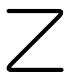
\includegraphics[keepaspectratio]{images/part002_816cd56c.jpg}}

(VI, p.~271, th. 1) (which we have denoted \(u(\mathrm{D})\) in VI, p.~271), the series of complex terms with general term \(\alpha_{n}\lambda^{n+p}\) is not necessarily convergent for \(\lambda \neq 0\) , and that even if it converges for certain values of \(\lambda\) , the sum is not necessarily equal to the indicatrix \(u(\lambda)\) of U (VI, p.~291, exerc. 2). We shall say that the composition operator U is regular if there exists a neighbourhood of 0 in C such that the series with general term \(\alpha_{n}\lambda^{n+p}\) is absolutely convergent and has sum equal to the indicatrix \(u(\lambda)\) on this neighbourhood \(^{1}\) . Let us apply formula (27) of VI, p.~278, to the function \(e^{\lambda x}\) , making h = 0; since \(\mathrm{D}^{m}(e^{\lambda x}) = \lambda^{m} e^{\lambda x}\) one has \(U_{0}^{\xi}\left(\mathrm{D}^{m}(e^{\lambda x})\right) = \lambda^{m} u(\lambda)\) ; it then follows that for every complex \(\lambda\) such that \(u(\lambda) \neq 0\)

\[
\frac {\lambda^ {p} e ^ {\lambda x}}{u (\lambda)} = \sum_ {m = 0} ^ {n} u _ {m} (x) \frac {\lambda^ {m}}{m !} - \frac {\lambda^ {n + 1}}{u (\lambda)} U _ {0} ^ {\xi} \left(\int_ {0} ^ {\xi - x} \frac {1}{n !} u _ {n} (x + \eta) e ^ {\lambda (\xi - \eta)} d \eta\right)\tag{31}
\]

and in particular, for \(x = 0\)

\[
\frac {\lambda^ {p}}{u (\lambda)} = \sum_ {m = 0} ^ {n} \beta_ {m} \frac {\lambda^ {m}}{m !} - \frac {\lambda^ {n + 1}}{u (\lambda)} U _ {0} ^ {\xi} \left(\int_ {0} ^ {\xi} \frac {1}{n !} u _ {n} (\eta) e ^ {\lambda (\xi - \eta)} d \eta\right)\tag{32}
\]

with \(\beta_{m} = u_{m}(0)\) .

If \(U\) is a regular operator, for all \(\lambda \in \mathbf{C}\) such that the entire series \(u(\lambda) = \sum_{n=0}^{\infty} \alpha_n \lambda^{n+p}\) and \(\sum_{n=0}^{\infty} \beta_n \frac{\lambda^n}{n!}\) are absolutely convergent \(^2\) , it follows from formula (16) and the formula for the product of two absolutely convergent series (Gen.~Top., VIII, p.~115, prop. 1) that one has

\[
{\frac {\lambda^ {p}}{u (\lambda)}} = \sum_ {n = 0} ^ {\infty} \beta_ {n} {\frac {\lambda^ {n}}{n !}}.\tag{33}
\]

Similarly, since the Taylor expansion of \(e^{\lambda x}\) is absolutely convergent for every \(\lambda \in \mathbf{C}\) and every \(x \in \mathbf{C}\) (III, p.~106) one also has (formulae (6) (VI, p.~273) and (16) (VI, p.~274)), for all the values considered and for all \(x \in \mathbf{C}\)

\[
\frac {\lambda^ {p} e ^ {\lambda x}}{u (\lambda)} = \sum_ {n = 0} ^ {\infty} u _ {n} (x) \frac {\lambda^ {n}}{n !}.\tag{34}
\]

Remark. One can use formula (33) (resp. (34)) to calculate the \(\beta_{n}\) (resp. the \(u_{n}(x)\) ) by using the following lemma on entire series:

Lemma. If two entire series \(\sum_{n=0}^{\infty} c_n \lambda^n\) , \(\sum_{n=0}^{\infty} d_n \lambda^n\) are absolutely convergent for all \(\lambda\) in a neighbourhood of 0, and if \(\sum_{n=0}^{\infty} c_n \lambda^n = \sum_{n=0}^{\infty} d_n \lambda^n\) for these values of \(\lambda\) , then \(c_n = d_n\) for all integers \(n \geqslant 0^3\) .

If, by any procedure, one can find an entire series that converges to \(\lambda^p / u(\lambda)\) on a neighbourhood of 0, then the coefficients of this series are necessarily equal to the \(\beta_n / n!\) . It is this procedure that we shall apply in the examples that follow.

Examples. 1) If \(U\) is the identity map one has \(u(\lambda) = 1\) and the operator \(U\) is clearly regular; since \(u_{n}(x) = x^{n}\) the formula (27) of VI, p.~278, can be written, putting \(t = \xi - \eta\)

\[
f (x + h) = \sum_ {n = 0} ^ {\infty} \frac {1}{m !} f ^ {(m)} (h) x ^ {m} + \int_ {h} ^ {x + h} f ^ {(n + 1)} (t) \frac {(x + h - t) ^ {n}}{n !} d t
\]

that is, it reduces to the Taylor formula (II, p.~62).

\begin{enumerate}
\def\labelenumi{\arabic{enumi})}
\setcounter{enumi}{1}
\tightlist
\item
  Let us take for U the composition operator which, to every function f defined on \(R_{+}\) , associates the function \(x \mapsto f(x + 1) - f(x)\) ; then
\end{enumerate}

\[
U _ {x} ^ {\xi} (f (\xi)) = f (x + 1) - f (x);
\]

we have seen (VI, p.~275) that the restriction of U to C{[}X{]} is equal to \(e^{D}-1\) . Since, on the other hand, \(u(\lambda)=e^{\lambda}-1\) , the operator U is regular; we shall see (VI, p.~288) how to determine the Bernoulli numbers \(b_{n}\) by calculating an expansion of \(\frac{\lambda}{e^{\lambda}-1}\) as a convergent entire series. On applying formula (27) of VI, p.~278 to a primitive of a function f admitting a continuous \(n^{th}\) derivative on \(R_{+}\) , we obtain

\[
\begin{array}{l} f (x + h) = \int_ {h} ^ {h + 1} f (t) d t \\ \qquad + \sum_ {m = 1} ^ {n} \frac {1}{m !} \mathrm{B} _ {m} (x) \left(f ^ {(m - 1)} (h + 1) - f ^ {(m - 1)} (h)\right) + \mathrm{R} _ {n} (x, h) \end{array}\tag{35}
\]

\[
\begin{array}{l} \mathrm{R} _ {n} (x, h) = - \int_ {0} ^ {1 - x} \frac {\mathrm{B} _ {n} (x + \eta)}{n !} f ^ {(n)} (h + 1 - \eta) d \eta \\ \qquad \qquad + \int_ {0} ^ {- x} \frac {\mathrm{B} _ {n} (x + \eta)}{n !} f ^ {(n)} (h - \eta) d \eta . \end{array}\tag{36}
\]

*3) Let \(\mathbf{E}\) be the vector space of functions \(f\) defined and continuous on \(\mathbf{R}\) , and such that the integral \(\int_{-\infty}^{+\infty} f(x + \xi)e^{-\xi^2 / 2}d\xi\) converges for all \(x \geqslant 0\) . The operator \(\mathrm{U}\) defined by

\[
U _ {x} ^ {\xi} (f (\xi)) = \frac {1}{\sqrt {2 \pi}} \int_ {- \infty} ^ {+ \infty} e ^ {- \xi^ {2} / 2} f (x + \xi) d \xi
\]

is then defined on E and is clearly a composition operator. The space E contains all the exponentials \(e^{\lambda x}\) ( \(\lambda\) arbitrary complex), and one has

\[
\begin{array}{l} u (\lambda) = \frac {1}{\sqrt {2 \pi}} \int_ {- \infty} ^ {+ \infty} e ^ {- (\xi^ {2} / 2) + \lambda \xi} d \xi \\ = \frac {1}{\sqrt {2 \pi}} e ^ {\lambda^ {2} / 2} \int_ {- \infty} ^ {+ \infty} e ^ {- (\xi - \lambda) ^ {2} / 2} d \xi = e ^ {\lambda^ {2} / 2} \end{array}
\]

(cf.~III, p.~120, exerc. 24, and VII, p.~313, formula (22)). One has \(n! \alpha_n = U_0^\xi (\xi^n) = \frac{1}{\sqrt{2\pi}} \int_{-\infty}^{+\infty} e^{-\xi^2 / 2} \xi^n d\xi\) . For every integer \(n\) one can write

\[
\sum_ {k = 0} ^ {n} \int_ {- \infty} ^ {+ \infty} \frac {| \lambda \xi | ^ {k}}{k !} e ^ {- \xi^ {2} / 2} d \xi \leqslant 2 \int_ {0} ^ {+ \infty} e ^ {- (\xi^ {2} / 2) + | \lambda | \xi} d \xi .
\]

The series \(\sum_{n=0}^{\infty}e^{-\xi^{2}/2}\frac{(\lambda\xi)^{n}}{n!}\) can therefore be integrated term-by-term over R (II, p.~72, cor. 1), which proves that the series \(\sum_{n=0}^{\infty}\alpha_{n}\lambda^{n}\) converges absolutely for every \(\lambda\in C\) , and has a sum equal to \(u(\lambda)=e^{\lambda^{2}/2}=\sum_{n=0}^{\infty}\frac{\lambda^{2n}}{2^{n}n!}\) ; thus the operator U is regular. Applying the lemma mentioned above shows that \(\alpha_{2n}=1/2^{n}n!\) , \(\alpha_{2n+1}=0\) for every \(n\geqslant0\) ; the operator U is thus of order 0. One has

\[
\frac {1}{u (\lambda)} = e ^ {- \lambda^ {2} / 2} = \sum_ {n = 0} ^ {\infty} \frac {(- 1) ^ {n} \lambda^ {2 n}}{2 ^ {n} n !},
\]

the series being absolutely convergent for every \(\lambda \in \mathbf{C}\) ; another application of the lemma shows that \(\beta_{2n} = \frac{(-1)^n}{2^n}\frac{(2n)!}{n!}\) , \(\beta_{2n+1} = 0\) ; further, the series \(\sum_{n=0}^{\infty}\frac{\lambda^n}{n!} u_n(x)\) is absolutely convergent for every \(\lambda \in \mathbf{C}\) and every \(x \in \mathbf{R}\) , and one has

\[
\sum_ {n = 0} ^ {\infty} \frac {\lambda^ {n}}{n !} u _ {n} (x) = \exp \left(- \frac {\lambda^ {2}}{2} + \lambda x\right) = \exp \left(\frac {x ^ {2}}{2}\right) \exp \left(- \frac {1}{2} (\lambda - x) ^ {2}\right).
\]

On applying the Taylor formula to the function \(\exp(-x^2/2)\) one then obtains the following expression for the polynomials \(u_n(x)\) :

\[
u _ {n} (x) = (- 1) ^ {n} e ^ {x ^ {2} / 2} \frac {d ^ {n}}{d x ^ {n}} (e ^ {- x ^ {2} / 2}).
\]

This polynomial is called the Hermite polynomial of degree n, and is often denoted by \(\mathrm{H}_{n}(x)\) . The formulae (7), (8) and (9) of VI, p.~273, here give

\[
\frac {d \mathrm{H} _ {n}}{d x} = n \mathrm{H} _ {n - 1} (x)
\]

\[
\mathrm{H} _ {n} (x + y) = \sum_ {k = 0} ^ {n} {\binom {n} {k}} \mathrm{H} _ {n - k} (x)   y ^ {k}
\]

\[
\frac {1}{\sqrt {2 \pi}} \int_ {- \infty} ^ {+ \infty} e ^ {- \xi^ {2} / 2} \mathrm{H} _ {n} (x + \xi) d \xi = x ^ {n}
\]

and the formula (27) of VI, p.~278, becomes, for \(h = 0\)

\[
\begin{array}{l} \sqrt {2 \pi} f (x) = \sum_ {m = 0} ^ {n} \left(\int_ {- \infty} ^ {+ \infty} e ^ {- \xi^ {2} / 2} f ^ {(m)} (\xi) d \xi\right) \frac {\mathrm{H} _ {m} (x)}{m !} \\ - \int_ {- \infty} ^ {+ \infty} d \xi \int_ {0} ^ {\xi} \frac {\mathrm{H} _ {n} (x + \eta)}{n !} e ^ {- (\xi + x) ^ {2} / 2} f ^ {(n + 1)} (x + \xi - \eta) d \eta . * \end{array}
\]

\subsection{THE EULER-MACLAURIN SUMMATION FORMULA}

In the formula (35) of VI, p.~280, let us replace x by 0 and h by x; since \(\mathrm{B}_{m}(0)=b_{m}\) it follows from the relations (24) of VI, p.~276, that for each integer p\textgreater0 one can write

\[
\begin{array}{l} f (x) = \int_ {x} ^ {x + 1} f (t) d t - \frac {1}{2} \big (f (x + 1) - f (x) \big) \\ \qquad + \sum_ {k = 1} ^ {p} \frac {b _ {2 k}}{(2 k) !} \left(f ^ {(2 k - 1)} (x + 1) - f ^ {(2 k - 1)} (x)\right) + \mathrm{R} _ {p} (x) \end{array}\tag{37}
\]

with

\[
\mathrm{R} _ {p} (x) = - \frac {1}{(2 p + 1) !} \int_ {0} ^ {1} \mathrm{B} _ {2 p + 1} (t) f ^ {(2 p + 1)} (x + 1 - t) d t.\tag{38}
\]

In this formula let us successively replace \(x\) by \(x + 1, x + 2, \ldots, x + n\) , and combine the formulae obtained, one by one; we obtain

\[
\left\{ \begin{array}{l} f (x) + f (x + 1) + \dots + f (x + n) \\ = \int_ {x} ^ {x + n + 1} f (t) d t - \frac {1}{2} \bigl (f (x + n + 1) - f (x) \bigr) \\ \quad + \sum_ {k = 1} ^ {p} \frac {b _ {2 k}}{(2 k) !} \bigl (f ^ {(2 k - 1)} (x + n + 1) - f ^ {(2 k - 1)} (x) \bigr) + \mathrm{T} _ {p} (x, n) \end{array} \right.\tag{39}
\]

with

\[
\mathrm{T} _ {p} (x, n) = - \frac {1}{(2 p + 1) !} \int_ {0} ^ {1} \mathrm{B} _ {2 p + 1} (t) \left(\sum_ {k = 0} ^ {n} f ^ {(2 p + 1)} (x + k + 1 - t)\right) d t.\tag{40}
\]

The remainder \(T_{p}(x,n)\) in this formula can be rewritten in the following way: denote by \(\overline{\mathbf{B}}_{2p+1}(t)\) the periodic function with period 1 which is equal to \(\mathbf{B}_{2p+1}(t)\) on the interval {[}0, 1{[}. Then

\[
\int_ {0} ^ {1} \mathrm{B} _ {2 p + 1} (t) f ^ {(2 p + 1)} (x + k + 1 - t) d t = \int_ {k} ^ {k + 1} \overline {{\mathrm{B}}} _ {2 p + 1} (1 - s) f ^ {(2 p + 1)} (x + s) d s
\]

and consequently

\[
\mathrm{T} _ {p} (x, n) = - \frac {1}{(2 p + 1) !} \int_ {0} ^ {n + 1} \overline {{\mathrm{B}}} _ {2 p + 1} (1 - s) f ^ {(2 p + 1)} (x + s) d s.\tag{41}
\]

The formula (39) is called the Euler-Maclaurin summation formula; it is applicable to every complex function having a continuous \((2p+1)^{th}\) derivative on an interval \([x_{0},+\infty[\) , for every \(x\geqslant x_{0}\) . We shall see (VI, p.~288) how to estimate the remainder \(T_{p}(x,n)\) in this formula.

\section{EULERIAN EXPANSIONS OF THE TRIGONOMETRIC FUNCTIONS AND BERNOULLI NUMBERS}

\subsection{\texorpdfstring{EULERIAN EXPANSION OF \(\cot z\)}{EULERIAN EXPANSION OF COT Z}}

By formula (20) of VI, p.~275, the numbers \(b_{n} / n!\) are the coefficients in the expansion of \(S / (e^{S} - 1)\) as a formal series; we shall show in this section that the function \(z / (e^{z} - 1)\) is equal to the sum of an absolutely convergent entire series on a neighbourhood of 0 in \(\mathbf{C}\) ; it will follow from the lemma of VI, p.~280, that the coefficients of this series are the numbers \(b_{n} / n!\) , from which we shall deduce estimates for the Bernoulli numbers \(b_{n}\) .

In the first place we note that

\[
{\frac {z}{e ^ {z} - 1}} = - {\frac {z}{2}} + {\frac {z}{2}} {\frac {e ^ {z} + 1}{e ^ {z} - 1}} = - {\frac {z}{2}} + {\frac {i z}{2}} \cot {\frac {i z}{2}}.\tag{1}
\]

We shall obtain below a series expansion for \(\cot z\) , valid for every \(z\) not an integer multiple of \(\pi\) .

PROPOSITION 1. For every complex number \(z\) and every integer \(n\) one has

\[
\sin n z = 2 ^ {n - 1} \sin z \sin \left(z + \frac {\pi}{n}\right) \sin \left(z + \frac {2 \pi}{n}\right) \dots \sin \left(z + \frac {(n - 1) \pi}{n}\right).\tag{2}
\]

Indeed, one can write

\[
\begin{array}{l} \sin n z = \frac {e ^ {n i z} - e ^ {- n i z}}{2 i} = \frac {e ^ {- n i z} (e ^ {2 n i z} - 1)}{2 i} \\ \quad = \frac {e ^ {- n i z} (e ^ {2 i z} - 1) (e ^ {2 i z} - e ^ {- 2 i \pi / n}) \dots (e ^ {2 i z} - e ^ {- 2 (n - 1) i \pi / n})}{2 i} \\ \quad = A \sin z \sin \left(z + \frac {\pi}{n}\right) \sin \left(z + \frac {2 \pi}{n}\right) \dots \sin \left(z + \frac {(n - 1) \pi}{n}\right) \end{array}
\]

with

\[
\mathrm{A} = (2 i) ^ {n - 1} e ^ {- \frac {i \pi}{n} (1 + 2 + \dots + (n - 1))} = (2 i) ^ {n - 1} e ^ {- i (n - 1) \frac {\pi}{2}} = 2 ^ {n - 1}.
\]

COROLLARY 1. For every integer n one has

\[
\sin \frac {\pi}{n} \sin \frac {2 \pi}{n} \dots \sin \frac {(n - 1) \pi}{n} = \frac {n}{2 ^ {n - 1}}.\tag{3}
\]

It suffices to divide both sides of (2) by \(\sin z\) and let z tend to 0.

COROLLARY 2. For every odd integer \(n = 2m + 1\) , and every complex number z such that nz is not an integral multiple of \(\pi\) , one has

\[
\cot n z = (- 1) ^ {m} \cot z \cot \left(z + \frac {\pi}{n}\right) \dots \cot \left(z + \frac {(n - 1) \pi}{n}\right).\tag{4}
\]

Indeed, \(\sin n\left(z + \frac{\pi}{2}\right) = \sin \left(nz + \frac{\pi}{2} + m\pi\right) = (-1)^m\cos nz\) , whence, replacing \(z\) by \(z + \frac{\pi}{2}\) in (2),

\[
\cos n z = (- 1) ^ {m} 2 ^ {n - 1} \cos z \cos \left(z + \frac {\pi}{n}\right) \dots \cos \left(z + \frac {(n - 1) \pi}{n}\right)\tag{5}
\]

and the formulae (2) and (5) give (4) on division term-by-term when \(\sin nz \neq 0\) .

In all that follows we shall always assume that \(n = 2m + 1\) is an odd integer; the formula (4) can also be written

\[
\cot n z = (- 1) ^ {m} \prod_ {k = - m} ^ {m} \cot \left(z - \frac {k \pi}{n}\right).
\]

For, one has

\[
\cot \left(z - \frac {k \pi}{n}\right) = \frac {1 + \tan z \tan \frac {k \pi}{n}}{\tan z - \tan \frac {k \pi}{n}}
\]

for \(\tan z\) finite; \(\cot nz\) is thus a rational function in \(u = \tan z\) , whose numerator is of degree n - 1, and whose denominator, of degree n, has the n simple roots \(\tan k\pi/n\) ; decomposing this into simple fractions yields

\[
\cot n z = \sum_ {k = - m} ^ {m} \frac {\mathrm{A} _ {k}}{u - \tan \frac {k \pi}{n}}\tag{6}
\]

where

\[
\begin{array}{l}\mathrm{A} _ {k} = \lim _ {z \rightarrow k \pi / n} \cot n z \left(\tan z - \tan \frac {k \pi}{n}\right) = \lim _ {z \rightarrow k \pi / n} \frac {\cos n z}{\sin n z} \frac {\sin \left(z - \frac {k \pi}{n}\right)}{\cos z \cos \frac {k \pi}{n}}\\= \lim _ {h \rightarrow 0} \frac {\cos n h}{\cos \frac {k \pi}{n} \cos \left(h + \frac {k \pi}{n}\right)} \frac {\sin h}{\sin n h} = \frac {1}{n \cos^ {2} \frac {k \pi}{n}}\end{array}
\]

whence, on isolating the term in (6) corresponding to k = 0 and combining the terms corresponding to opposite values of k, and replacing z by z/n,

\[
\cot z = \frac {1}{n \tan \frac {z}{n}} + \sum_ {k = 1} ^ {m} \frac {2 n \tan \frac {z}{n}}{\cos^ {2} \frac {k \pi}{n} \left(n \tan \frac {z}{n}\right) ^ {2} - \left(n \sin \frac {k \pi}{n}\right) ^ {2}}\tag{7}
\]

valid for every complex number \(z\) not an integral multiple of \(\pi / 2\) . One can write this formula in the form

\[
\cot z = \frac {1}{n \tan \frac {z}{n}} + \sum_ {k = 1} ^ {\infty} v _ {k} (n, z)
\]

with \(v_{k}(n,z) = 0\) for \(k > m\) and

\[
v _ {k} (n, z) = \frac {2 n \tan \frac {z}{n}}{\cos^ {2} \frac {k \pi}{n} \left(n \tan \frac {z}{n}\right) ^ {2} - \left(n \sin \frac {k \pi}{n}\right) ^ {2}}
\]

for \(1 \leqslant k \leqslant m\) . We shall see that for every \(z\) contained in a compact subset K of C, not containing any integral multiple of \(\pi\) , and for every sufficiently large odd \(n\) , the series with general term \(v_{k}(n,z)\) is normally convergent. Indeed, as \(n\) tends to \(+\infty\) , \(\tan \frac{z}{n}\) tends to \(\frac{z}{n}\) uniformly on K, so there exists a number M \textgreater{} 0 such that \(\left| n \tan \frac{z}{n} \right| \leqslant M\) for every sufficiently large \(m\) and every \(z \in K\) . On the other hand, for \(0 \leqslant x \leqslant \pi/2\) one has \(\sin x/x \geqslant 1 - \frac{x^2}{6} \geqslant \frac{1}{2}\) , so for \(1 \leqslant k \leqslant m\) one has \(n \sin \frac{k\pi}{n} \geqslant k\pi/2\) ; consequently, when \(m\) is sufficiently large, for every integer \(k\) such that \(k\pi / 2 > \mathbf{M}\) one has \(|v_k(n, z)| \leqslant \frac{8\mathbf{M}}{k^2\pi^2 - 4\mathbf{M}^2}\) , which proves our assertion. For \(k\) fixed, \(v_k(n, z)\) tends (uniformly on \(\mathbf{K}\) ) to \(\frac{2z}{z^2 - k^2\pi^2}\) as \(n\) tends to \(+\infty\) . Consequently:

THEOREM 1. For every complex number z not an integral multiple of \(\pi\) one has

\[
\cot z = \frac {1}{z} + \sum_ {n = 1} ^ {\infty} \frac {2 z}{z ^ {2} - n ^ {2} \pi^ {2}}\tag{8}
\]

the series on the right being normally convergent on every compact subset \(K \subset C\) not containing any integer multiple of \(\pi\) (Eulerian expansion of \(\cot z\) ).

\subsection{EULERIAN EXPANSION OF sin z}

For every odd integer \(n = 2m + 1\) and complex \(z\) the formula (2) of VI, p.~283, can be written

\[
\begin{array}{l} \sin n z = (- 1) ^ {m}   2 ^ {n - 1}   \prod_ {k = - m} ^ {m}   \sin \left(z - \frac {k \pi}{n}\right) \\ = (- 1) ^ {m}   2 ^ {n - 1}   \sin z   \prod_ {k = 1} ^ {m}   \sin \left(z - \frac {k \pi}{n}\right) \sin \left(z + \frac {k \pi}{n}\right). \end{array}
\]

Now, one has \(\sin\left(z-\frac{k\pi}{n}\right)\sin\left(z+\frac{k\pi}{n}\right)=\sin^{2}z-\sin^{2}\frac{k\pi}{n}\) , and, by (3) (VI, p.~284), \(\prod_{k=1}^{m}\sin^{2}\frac{k\pi}{n}=\frac{n}{2^{n-1}}\) , whence, on replacing \(z\) by \(z/n\) ,

\[
\sin z = n \sin \frac {z}{n} \prod_ {k = 1} ^ {m} \left(1 - \frac {\sin^ {2} \frac {z}{n}}{\sin^ {2} \frac {k \pi}{n}}\right).\tag{9}
\]

One can write this formula as \(\sin z = n\sin \frac{z}{n}\prod_{k = 1}^{m}\big(1 - w_k(n,z)\big)\) , with \(w_{k}(n,z) = 0\) for \(k > m\) and \(w_{k}(n,z) = \frac{\sin^{2}\frac{z}{n}}{\sin^{2}\frac{k\pi}{n}}\) for \(1\leqslant k\leqslant m\) . We shall see that for every \(z\) contained in a compact subset \(\mathbf{K}\) of \(\mathbf{C}\) , and for \(n\) odd, the series with general term \(w_{k}(n,z)\) is normally convergent. Indeed, as \(n\) tends to \(+\infty\) , \(n\sin \frac{z}{n}\) tends uniformly to \(z\) on \(\mathbf{K}\) , so there exists a number \(\mathbf{M} > 0\) such that \(\left|n\sin \frac{z}{n}\right|\leqslant \mathbf{M}\) for every integer \(m\) and every \(z\in \mathbf{K}\) . We saw, moreover, in the proof of th. 1 of VI, p.~286, that for

\(1 \leqslant k \leqslant m\) one has \(n \sin \frac{k\pi}{n} \geqslant \frac{k\pi}{2}\) ; thus for every integer \(k\) such that \(k\pi/2 \geqslant M\) one has \(|w_k(n, z)| \leqslant 4M^2/k^2\pi^2\) , which proves our assertion. Since, for every fixed \(k\) , \(w_k(n, z)\) tends (uniformly on K) to \(z^2/k^2\pi^2\) as \(n\) tends to \(+\infty\) , one sees that:

THEOREM 2. For every complex number \(z\) one has

\[
\sin z = z \prod_ {n = 1} ^ {\infty} \left(1 - \frac {z ^ {2}}{n ^ {2} \pi^ {2}}\right)\tag{10}
\]

the infinite product on the right being absolutely and uniformly convergent on every compact subset of C (Eulerian expansion of \(\sin z\) ).

\subsection{APPLICATION TO THE BERNOULLI NUMBERS}

Theorem 1 of VI, p.~286, shows that, for \(0 \leqslant x < \pi\) , the series with general term \(\frac{2x}{n^2\pi^2 - x^2} \geqslant 0\) converges. On the other hand, one can write, for every complex number \(z\) such that \(|z| < \pi\) ,

\[
{\frac {2 z}{n ^ {2} \pi^ {2} - z ^ {2}}} = {\frac {2 z}{n ^ {2} \pi^ {2}}} \sum_ {k = 0} ^ {\infty} {\frac {z ^ {2 k}}{n ^ {2 k} \pi^ {2 k}}}
\]

the series on the right being absolutely convergent. We shall deduce from this that the ``double'' series

\[
\sum_ {n = 1} ^ {\infty} \sum_ {k = 1} ^ {\infty} \frac {- 2 z ^ {2 k - 1}}{n ^ {2 k} \pi^ {2 k}}\tag{11}
\]

is absolutely convergent in the open disc \(|z| < \pi\) , normally convergent on every compact set contained in this disc, and has sum \(\cot z - \frac{1}{z}\) . Indeed, for \(|z| \leqslant a < \pi\) the absolute value of the general term of (11) is at most equal to \(2a^{2k-1}/n^{2k}\pi^{2k}\) , and the sum of any finite number of the terms \(2a^{2k-1}/n^{2k}\pi^{2k}\) is less than the finite number \(\sum_{n=1}^{\infty} \frac{2a}{n^2\pi^2 - a^2}\) ; on summing first over \(k\) , then over \(n\) , one sees that the sum of the series (11) is equal to \(\sum_{n=1}^{\infty} \frac{2z}{z^2 - n^2\pi^2}\) , which proves our statement.

If now one sums the series (11) first over \(n\) and then over \(k\) one obtains the identity (for \(|z| < \pi\) )

\[
\cot z - \frac {1}{z} = - 2 \sum_ {k = 1} ^ {\infty} \frac {S _ {2 k}}{\pi^ {2 k}} z ^ {2 k - 1}\tag{12}
\]

where we have put \(S_{k} = \sum_{n=1}^{\infty} \frac{1}{n^{k}}\) . By (1) (VI, p.~283) one thus has, for \(|z| < 2\pi\)

\[
\frac {z}{e ^ {z} - 1} = 1 - \frac {z}{2} + \sum_ {n = 1} ^ {\infty} \frac {(- 1) ^ {n - 1} S _ {2 n}}{2 ^ {2 n - 1} \pi^ {2 n}} z ^ {2 n}\tag{13}
\]

whence we obtain the formula

\[
b _ {2 n} = (- 1) ^ {n - 1} (2 n)! \frac {2 \mathrm{S} _ {2 n}}{(2 \pi) ^ {2 n}} \quad \text {   for   } n \geqslant 1,\tag{14}
\]

a formula which shows in particular that the numbers \(S_{2n} / \pi^{2n}\) are rational. Clearly \(S_{k + 1} \leqslant S_k\) so, for every integer \(k \geqslant 2\) , we have \(S_k \leqslant S_2 = \pi^2 / 6 \leqslant 2\) ; from (14) one deduces the following inequalities for the Bernoulli numbers

\[
\frac {2 (2 n) !}{(2 \pi) ^ {2 n}} \leqslant | b _ {2 n} | \leqslant 4 \frac {(2 n) !}{(2 \pi) ^ {2 n}} \quad \text {   for   } n \geqslant 1.\tag{15}
\]

From these inequalities one can deduce an estimate for the Bernoulli polynomial \(\mathrm{B}_n(x) = \sum_{k=0}^{n}\binom{n}{k}b_kx^{n - k}\) ; in particular, for \(0 \leqslant x \leqslant 1\) one has

\[
\left| \mathrm{B} _ {n} (x) \right| \leqslant 4 \sum_ {k = 0} ^ {n} \binom {n} {k} \frac {k !}{(2 \pi) ^ {k}} = 4 \frac {n !}{(2 \pi) ^ {n}} \sum_ {k = 0} ^ {n} \frac {(2 \pi) ^ {k}}{k !} \leqslant 4 e ^ {2 \pi} \frac {n !}{(2 \pi) ^ {n}}.\tag{16}
\]

\section{BOUNDS FOR THE REMAINDER IN THE EULER-MACLAURIN SUMMATION FORMULA}

\subsection{BOUNDS FOR THE REMAINDER IN THE EULER-MACLAURIN SUMMATION FORMULA}

The estimate obtained in (16) for the Bernoulli polynomials on the interval \([0, 1]\) allows one to estimate the remainder \(T_{p}(x, n)\) in the Euler-Maclaurin summation formula (VI, p.~282, formula (39)) easily:

\[
\left\{ \begin{array}{l} f (x) + f (x + 1) + \dots + f (x + n) \\ = \int_ {x} ^ {x + n + 1} f (t) d t - \frac {1}{2} \bigl (f (x + n + 1) - f (x) \bigr) \\ \qquad + \sum_ {k = 1} ^ {p} \frac {b _ {2 k}}{(2 k) !} \bigl (f ^ {(2 k - 1)} (x + n + 1) - f ^ {(2 k - 1)} (x) \bigr) + T _ {p} (x, n). \end{array} \right.\tag{1}
\]

Indeed, one has (VI, p.~283, formula (41))

\[
\mathrm{T} _ {p} (x, n) = - \frac {1}{(2 p + 1) !} \int_ {0} ^ {n + 1} \overline {{\mathrm{B}}} _ {2 p + 1} (1 - s) f ^ {(2 p + 1)} (x + s) d s\tag{2}
\]

where \(\overline{\mathbf{B}}_{2p + 1}(t)\) is the periodic function of period 1 equal to \(\mathrm{B}_{2p + 1}(t)\) on the interval {[}0, 1{[}. The formula (16) of VI, p.~288, shows that

\[
\left| \overline {{{{\mathrm{B}}}}} _ {2 p + 1} (t) \right| \leqslant 4 e ^ {2 \pi} \frac {(2 p + 1) !}{(2 \pi) ^ {2 p + 1}}\tag{3}
\]

for all \(t \in R\) , and applying the mean value formula gives the estimate

\[
\left| \mathrm{T} _ {p} (x, n) \right| \leqslant \frac {4 e ^ {2 \pi}}{(2 \pi) ^ {2 p + 1}} \int_ {x} ^ {x + n + 1} \left| f ^ {(2 p + 1)} (t) \right| d t\tag{4}
\]

for \(\mathrm{T}_p(x,n)\) .

\subsection{APPLICATION TO ASYMPTOTIC EXPANSIONS}

The Euler-Maclaurin formula allows one to give a more complete solution (in the most important cases) to the problem treated in V, p.~238 to 242, that of obtaining an asymptotic expansion of the partial sum \(s_n = \sum_{m=0}^{n} g(m)\) (resp. of the remainder \(r_n = \sum_{m=n+1}^{\infty} g(m)\) ), where \(g\) is a scalar function, \(> 0\) , monotone, defined on \([0, +\infty[\) .

We shall restrict ourselves to the case where g is an (H) function (V, p.~252), of order 0 relative to \(e^{x}\) ; in other words, one has the relation \(g' \ll g\) ; from this relation one deduces \(g^{(k+1)} \ll g^{(k)}\) for every integer k \textgreater{} 0 such that none of the derivatives \(g^{(h)}\) of order \(h \leqslant k\) is equivalent to a constant (V, p.~232, prop. 7). Let p be an integer such that none of the derivatives \(g^{(h)}\) of order \(h \leqslant 2p\) is equivalent to a constant. First we assume that the series with general term \(g(n)\) has infinite sum, and distinguish several cases:

\(1^{\circ}\left|g^{(2p - 1)}(n)\right|\) tends to \(+\infty\) with \(n\) ; we have the same, by the hypothesis, for \(\left|g^{(2k - 1)}(n)\right|\) for \(1\leqslant k\leqslant p\) ; further, since \(g^{(2p + 1)}\) is monotone on a neighbourhood of \(+\infty\) , the formula (4) of VI, p.~289, gives \(\mathrm{T}_p(0,n) = O\big(g^{(2p)}(n + 1)\big) = o\big(g^{(2p - 1)}(n + 1)\big)\) ; the Euler-Maclaurin formula, applied for \(x = 0\) , shows that

\[
\begin{array}{l} s _ {n} = \sum_ {m = 0} ^ {n} g (m) = \int_ {0} ^ {n + 1} g (t) d t - \frac {1}{2} g (n + 1) \\ \qquad + \sum_ {k = 1} ^ {p} \frac {b _ {2 k}}{(2 k) !} g ^ {(2 k - 1)} (n + 1) + o \big (g ^ {(2 p - 1)} (n + 1) \big) \end{array}
\]

each of the terms of this sum being negligible relative to the preceding one; on expanding each of them relative to a comparison scale E one will then have an asymptotic expansion for \(s_{n}\) .

\(2^{\circ}\) Now suppose that for an index \(q\) such that \(1 \leqslant q \leqslant p\) we have \(\left|g^{(2q-1)}(n)\right|\) tending to \(+\infty\) with \(n\) , but that \(g^{(2k-1)}(n)\) tends to 0 for \(k > q\) . Since \(g^{(2p+1)}\) is monotone on a neighbourhood of \(+\infty\) the integral \(\int_0^\infty \left|g^{(2p+1)}(u)\right| du\) converges, and one can then write

\[
\begin{array}{l} s _ {n} = \sum_ {m = 0} ^ {n} g (m) = \int_ {0} ^ {n + 1} g (t) d t - \frac {1}{2} g (n + 1) + \sum_ {k = 1} ^ {q} \frac {b _ {2 k}}{(2 k) !} g ^ {(2 k - 1)} (n + 1) + C \\ \qquad + \sum_ {k = q + 1} ^ {p} \frac {b _ {2 k}}{(2 k) !} g ^ {(2 k - 1)} (n + 1) + o \big (g ^ {(2 p - 1)} (n + 1) \big) \end{array}
\]

where C is a constant: indeed

\[
\int_ {n + 1} ^ {\infty} \left| g ^ {(2 p + 1)} (u) \right| d u = O \big (g ^ {(2 p)} (n + 1) \big) = o \big (g ^ {(2 p - 1)} (n + 1) \big).
\]

The same formula is valid when \(g(n)\) itself tends to 0. Finally, when the series with general term \(g(n)\) converges one has, for the remainder \(r_n = \sum_{m=n+1}^{\infty} g(m)\) , the expansion

\[
\begin{array}{l} r _ {n} = \sum_ {m = n + 1} ^ {\infty} g (m) = \int_ {n + 1} ^ {\infty} g (t) d t + \frac {1}{2} g (n + 1) \\ \qquad - \sum_ {k = 1} ^ {p} \frac {b _ {2 k}}{(2 k) !} g ^ {(2 k - 1)} (n + 1) + o \big (g ^ {(2 p - 1)} (n + 1) \big). \end{array}
\]

\setcounter{exercisegroup}{0}
\refstepcounter{exercisegroup}
\section*{Exercises on \S\arabic{exercisegroup}}
\phantomsection
\addcontentsline{toc}{section}{Exercises on \protect\S\arabic{exercisegroup}}

\begin{enumerate}
\def\labelenumi{\arabic{enumi})}
\tightlist
\item
  Let \(\mathbf{K}\) be a field of characteristic 0, let \(U\) and \(V\) two composition operators in \(\mathrm{K}[\mathrm{X}]\) , and \(W = VU = UV\) ; let \((u_n), (v_n)(w_n)\) be the sequences of Appell polynomials corresponding to \(U, V, W\) respectively. Show that if \(p\) is the order of \(U\) then
\end{enumerate}

\[
w _ {n} ^ {(p)} (\mathrm{X}) = \sum_ {k = 0} ^ {n} \binom {n} {k} v _ {n - k} (\mathrm{X}) V _ {0} (u _ {k})
\]

\[
w _ {n} (\mathrm{X} + \mathrm{Y}) = \sum_ {k = 0} ^ {n} \binom {n} {k} u _ {k} (\mathrm{X}) v _ {n - k} (\mathrm{Y}).
\]

\begin{enumerate}
\def\labelenumi{\arabic{enumi})}
\setcounter{enumi}{1}
\tightlist
\item
  Let \(\mathbf{E}\) be the vector space over \(\mathbf{C}\) generated by the functions \(x^n\) ( \(n \in \mathbf{N}\) ), \(e^{\lambda x}\) ( \(\lambda \in \mathbf{C}\) , \(\lambda \neq 0\) ) and \(|x + \mu|\) ( \(\mu \in \mathbf{R}\) ).
\end{enumerate}

\begin{enumerate}
\def\labelenumi{\alph{enumi})}
\item
  Show that the preceding functions form a basis for E.
\item
  Let \(U\) be the composition operator defined on \(\mathbf{E}\) by the conditions: \(U_0^\xi (\xi^n) = (n!)^2\) , \(U(e^{\lambda x}) = e^{\lambda x}\) for \(\lambda \neq 0\) , \(U(|x + \mu|) = |x + \mu|\) for \(\mu \in \mathbf{R}\) . The indicatrix \(u(\lambda)\) is the constant 1 but the series with general term \(n!\lambda^n\) does not converge for any value \(\lambda \neq 0\) .
\item
  Let \(V\) be the composition operator defined on \(\mathbf{E}\) by the conditions \(V(x^n) = x^n\) , \(V(|x + \mu|) = |x + \mu|\) , \(V(e^{\lambda x}) = 0\) for \(\lambda \neq 0\) ; the indicatrix \(v(\lambda)\) is equal to 1 for \(\lambda = 0\) , to 0 for \(\lambda \neq 0\) , so is different from the sum of the series \(\sum_{n=0}^{\infty} \alpha_n \lambda^n\) where \(\alpha_n = V_0^\xi(\xi^n)/n!\) .
\item
  Let W be the composition operator defined on E by
\end{enumerate}

\[
W (x ^ {n}) = x ^ {n}, \qquad W (e ^ {\lambda x}) = e ^ {\lambda x}, \qquad W (| x + \mu |) = e ^ {x + \mu};
\]

show that \(VW \neq WV\) .

\begin{enumerate}
\def\labelenumi{\arabic{enumi})}
\setcounter{enumi}{2}
\tightlist
\item
  Let K be a field of characteristic 0. One says that an endomorphism U of the algebra \(K[X,Y]\) of polynomials in two indeterminates X, Y over K is a composition operator if, for every polynomial \(f \in K[X,Y]\) , one has, putting \(g = U(f)\) , that \(g(X + S, Y + T) = U_{X,Y}(f(X + S, Y + T))\) , where S and T are two other indeterminates.
\end{enumerate}

\begin{enumerate}
\def\labelenumi{\alph{enumi})}
\item
  Generalize prop. 1 and th. 1 to these operators. Derive a new proof of the formula \(e^{\mathrm{S + T}} = e^{\mathrm{S}}e^{\mathrm{T}}\) from this.
\item
  For composition operators of the form \(D_{X}^{p}D_{Y}^{q}u(D_{X},D_{Y})\) where the constant term of the formal series u is not zero, define the Appell polynomials \(u_{mn}\) and generalize props. 4, 5 and 6 of VI, p.~273 and 274.
\item
  Consider in particular the composition operator U defined by \(U(f(\mathrm{X},\mathrm{Y})) = f(\mathrm{X} + 1, \mathrm{Y} + 1) - f(\mathrm{X},\mathrm{Y} + 1) - f(\mathrm{X} + 1, \mathrm{Y}) + f(\mathrm{X},\mathrm{Y})\) ; the Appell polynomials corresponding to this operator are called Bernoulli polynomials and are denoted by \(B_{m,n}\) . Show that \(\mathrm{B}_{m,n}(\mathrm{X},\mathrm{Y}) = \mathrm{B}_{m}(\mathrm{X})\mathrm{B}_{n}(\mathrm{Y})\) .
\end{enumerate}

\setcounter{exercisegroup}{1}
\refstepcounter{exercisegroup}
\section*{Exercises on \S\arabic{exercisegroup}}
\phantomsection
\addcontentsline{toc}{section}{Exercises on \protect\S\arabic{exercisegroup}}

\begin{enumerate}
\def\labelenumi{\arabic{enumi})}
\tightlist
\item
  Establish the formulae
\end{enumerate}

\[
\tan z = \sum_ {n = 1} ^ {\infty} (- 1) ^ {n - 1} 2 ^ {2 n} (2 ^ {2 n} - 1) b _ {2 n} \frac {z ^ {2 n - 1}}{(2 n) !}
\]

\[
\frac {1}{\sin z} = \frac {1}{z} + \sum_ {n = 1} ^ {\infty} (- 1) ^ {n - 1} 2 (2 ^ {2 n - 1} - 1) b _ {2 n} \frac {z ^ {2 n - 1}}{(2 n) !}
\]

where the series on the right-hand sides converge absolutely, the first for \(|z| < \frac{\pi}{2}\) and the second for \(|z| < \pi\) (express \(\tan z\) and \(1/\sin 2z\) as linear combinations of \(\cot z\) and \(\cot 2z\) ). Deduce that the numbers \(\frac{2^{2n}(2^{2n}-1)}{2n} b_{2n}\) are integers. (Use the following lemma: if, in two absolutely convergent series \(\sum_{n=0}^{\infty} \alpha_n \frac{z^n}{n!}\) , \(\sum_{n=0}^{\infty} \beta_n \frac{z^n}{n!}\) the coefficients \(\alpha_n\) and \(\beta_n\) are integers, then, in their product written in the form \(\sum_{n=0}^{\infty} \gamma_n \frac{z^n}{n!}\) , the \(\gamma_n\) are integers.)

\begin{enumerate}
\def\labelenumi{\arabic{enumi})}
\setcounter{enumi}{1}
\tightlist
\item
  Establish the formula
\end{enumerate}

\[
(n - 1) \mathrm{B} _ {n} (\mathrm{X}) = n (\mathrm{X} - 1) \mathrm{B} _ {n - 1} (\mathrm{X}) - \sum_ {k = 0} ^ {n} \binom {n} {k} b _ {k}   \mathrm{B} _ {n - k} (\mathrm{X})
\]

(differentiate the series \(Se^{SX}/(e^{S}-1)\) with respect to S). Deduce the formula

\[
(2 n + 1) b _ {2 n} = - \sum_ {k = 1} ^ {n - 1} \binom {2 n} {2 k} b _ {2 k}   b _ {2 n - 2 k}
\]

for the Bernoulli numbers.

\begin{enumerate}
\def\labelenumi{\arabic{enumi})}
\setcounter{enumi}{2}
\tightlist
\item
  Show that, for every integer p \textgreater{} 1,
\end{enumerate}

\[
\mathrm{B} _ {n} \left(\frac {x}{p}\right) + \mathrm{B} _ {n} \left(\frac {x + 1}{p}\right) + \dots + \mathrm{B} _ {n} \left(\frac {x + p - 1}{p}\right) = \frac {1}{p ^ {n - 1}} \mathrm{B} _ {n} (\mathrm{X}).
\]

\begin{enumerate}
\def\labelenumi{\arabic{enumi})}
\setcounter{enumi}{3}
\tightlist
\item
  \begin{enumerate}
  \def\labelenumii{\alph{enumii})}
  \tightlist
  \item
    Prove the relation
  \end{enumerate}
\end{enumerate}

\[
\mathrm{B} _ {n} (1 - \mathrm{X}) = (- 1) ^ {n} \mathrm{B} _ {n} (\mathrm{X})
\]

(use the fact that \(b_{2n - 1} = 0\) for \(n > 1\) , and the relation

\[
\mathrm{B} _ {n} (1 - \mathrm{X}) - \mathrm{B} _ {n} (- \mathrm{X}) = (- 1) ^ {n} n \mathrm{X} ^ {n - 1}.
\]

\begin{enumerate}
\def\labelenumi{\alph{enumi})}
\setcounter{enumi}{1}
\tightlist
\item
  Show that
\end{enumerate}

\[
\mathrm{B} _ {n} \left(\frac {1}{2}\right) = b _ {n} \left(\frac {1}{2 ^ {n - 1}} - 1\right)
\]

(use exerc. 3).

\begin{enumerate}
\def\labelenumi{\alph{enumi})}
\setcounter{enumi}{2}
\tightlist
\item
  Show that, for n even, \(\mathrm{B}_{n}(\mathrm{X})\) has two roots in the interval {[}0, 1{]} of R, and that for n odd \textgreater{} 1, \(\mathrm{B}_{n}(\mathrm{X})\) has a simple root at the points 0, \(\frac{1}{2}\) and 1 and does not vanish at any other point of {[}0, 1{]} (use b) and the relation \(B_{n}^{\prime}=nB_{n-1}\) ).
\end{enumerate}

\(d\) ) Deduce from \(c\) ) that, for \(n\) even, the maximum of \(|\mathrm{B}_n(x)|\) on the interval {[}0, 1{]} is \(|b_n|\) , and that for \(n\) odd, if \(a_{n}\) is the maximum of \(|\mathrm{B}_n(x)|\) on {[}0, 1{]}, then

\[
\frac {4}{n + 1} \left| b _ {n + 1} \right| \left(1 - \frac {1}{2 ^ {n}}\right) \leqslant a _ {n} \leqslant \frac {1}{2} n \left| b _ {n - 1} \right|
\]

(use the mean value theorem).

\begin{enumerate}
\def\labelenumi{\arabic{enumi})}
\setcounter{enumi}{4}
\tightlist
\item
  If one puts \(S_{n}(x) = \frac{1}{n + 1} (\mathrm{B}_{n + 1}(x) - \mathrm{B}_{n + 1}(0))\) then, for every integer \(a > 0\) one has
\end{enumerate}

\[
\mathrm{S} _ {n} (a) = 1 ^ {n} + 2 ^ {n} + \dots + (a - 1) ^ {n}.
\]

\begin{enumerate}
\def\labelenumi{\alph{enumi})}
\item
  Show that for every integer \(n \geqslant 0\) and every integer \(a > 0\) one has \(2\mathrm{S}_{2n + 1}(a) \equiv 0 \pmod{a}\) (consider the sum \(k^{2n + 1} + (a - k)^{2n + 1}\) ).
\item
  If \(r\) and \(s\) are any two integers show that
\end{enumerate}

\[
\mathrm{S} _ {n} (r s) \equiv s \mathrm{S} _ {n} (r) + n r \mathrm{S} _ {n - 1} (r) \mathrm{S} _ {1} (s) \pmod {r ^ {2}}.
\]

\begin{enumerate}
\def\labelenumi{\alph{enumi})}
\setcounter{enumi}{2}
\tightlist
\item
  Let p be a prime number. Show that if n is divisible by p-1 one has \(S_{n}(p) \equiv -1 \pmod{p}\) , and if n is not divisible by p-1 then \(S_{n}(p) \equiv 0 \pmod{p}\) (if p does not divide the integer g remark that \(S_{n}(p) \equiv g^{n}S_{n}(p) \pmod{p}\) ).
\end{enumerate}

\begin{enumerate}
\def\labelenumi{\arabic{enumi})}
\setcounter{enumi}{5}
\tightlist
\item
  \begin{enumerate}
  \def\labelenumii{\alph{enumii})}
  \tightlist
  \item
    The rational numbers \(b_{n}\) having been defined by the formula (20) of VI, p.~275, one denotes by \(d_{n}\) the denominator \textgreater{} 0 of \(b_{n}\) written as an irreducible fraction. Show that no prime factor of \(d_{n}\) can be \(> n + 1\) (use the induction formula (23) of VI, p.~276).
  \end{enumerate}
\end{enumerate}

\begin{enumerate}
\def\labelenumi{\alph{enumi})}
\setcounter{enumi}{1}
\tightlist
\item
  Show that for every integer p \textgreater{} 0 and every integer n \textgreater{} 0
\end{enumerate}

\[
\mathrm{S} _ {n} (p) = b _ {n} p + \binom {n} {1} \frac {p}{2} b _ {n - 1} p + \dots + \binom {n} {r} \frac {p ^ {r}}{r + 1} b _ {n - r} p + \dots + \frac {p ^ {n + 1}}{n + 1}.
\]

\begin{enumerate}
\def\labelenumi{\alph{enumi})}
\setcounter{enumi}{2}
\item
  Deduce from b) by recursion on n that, for every prime number p the denominator of \(S_{n}(p) - b_{n}p\) written as an irreducible fraction, is not divisible by p (observe that \(p^{r+1}\) cannot divide \(r + 1\) ).
\item
  Deduce from c) that the number
\end{enumerate}

\[
b _ {n} - \sum_ {p} \frac {\mathrm{S} _ {n} (p)}{p}
\]

where \(p\) runs through the set of prime numbers \(p \leqslant n + 1\) and \(n\) is even, is an integer. Conclude that

\[
b _ {2 n} + \sum_ {p} \frac {1}{p}
\]

where \(p\) runs through the set of prime numbers such that \(p - 1\) divides \(2n\) , is an integer (Clausen-von Staudt theorem; use exerc. 5 c).

* 7) We accept that for every integer \(a > 0\) there are infinitely many prime numbers in the set of integers \(1 + ma\) ( \(m\) running through the set of integers \(\geqslant 1\) ; this is a particular case of Dirichlet's theorem on arithmetic progressions).

\begin{enumerate}
\def\labelenumi{\alph{enumi})}
\item
  Let n be an integer \(\geqslant 1\) , and let \(s \geqslant 1\) be an integer such that \(q = 1 + (2n + 1)!s\) is prime; show that if p is a prime number such that p - 1 divides 2nq then p - 1 must divide 2n (in the opposite case one would have p - 1 = qd with d an integer, and p would be divisible by \(d + 1\) ).
\item
  Deduce from a) that for every integer n \textgreater{} 0 there exist infinitely many integers m \textgreater{} n such that \(b_{2m} - b_{2n}\) is an integer.*
\end{enumerate}

\begin{enumerate}
\def\labelenumi{\arabic{enumi})}
\setcounter{enumi}{7}
\item
  Show that, for every prime number \(p > 3\) , \(\mathrm{S}_{2n}(p^k) - p^k b_{2n}\) , written as an irreducible fraction, has a numerator divisible by \(p^{2k}\) (argue as in exerc. 6).
\item
  To say that a rational number \(r\) is a \(p\) -adic integer (Gen.~Top., III, p.~322, exerc. 23) for \(p\) a prime number, means that when \(r\) is expressed as an irreducible fraction its denominator is not divisible by \(p\) ; one writes \(r \equiv 0 \pmod{p}\) to express the fact that \(r/p\) is a \(p\) -adic integer, and \(r \equiv r' \pmod{p}\) is equivalent by definition to \(r - r' \equiv 0 \pmod{p}\) .
\end{enumerate}

\begin{enumerate}
\def\labelenumi{\alph{enumi})}
\tightlist
\item
  Let \(m\) be a rational integer; the function \(F_{m}(z) = \frac{m}{e^{mz} - 1} - \frac{1}{e^{z} - 1}\) is analytic for \(|z|\) sufficiently small, so can be written as an entire series convergent on a neighbourhood of 0
\end{enumerate}

\[
\mathrm{F} _ {m} (z) = \sum_ {n = 1} ^ {\infty} (m ^ {n} - 1) \frac {b _ {n}}{n} \frac {z ^ {n - 1}}{(n - 1) !}.
\]

Show that also on a neighbourhood of 0

\[
\mathrm{F} _ {m} (z) = \sum_ {n = 0} ^ {\infty} c _ {n} (e ^ {z} - 1) ^ {n}
\]

where the \(c_{n}\) are \(p\) -adic integers; deduce that the numbers \(a_{n} = (m^{n} - 1)\frac{b_{n}}{n}\) are \(p\) -adic integers; further, one has \(a_{n + p - 1} \equiv a_{n} (\mathrm{mod.} p)\) .

\[
\frac {b _ {n + p - 1}}{n + p - 1} \equiv \frac {b _ {n}}{n} \pmod {p}
\]

\begin{enumerate}
\def\labelenumi{\alph{enumi})}
\setcounter{enumi}{1}
\tightlist
\item
  Deduce from a) that if \(p - 1\) does not divide \(n\) , then \(b_{n} / n\) is a \(p\) -adic integer and that (Kummer's congruences). (Take for \(m\) an integer whose class mod. \(p\) is a generator of the multiplicative group of the invertible elements of \(\mathbf{Z} / p\mathbf{Z}\) (Alg., VII. 12).)
\end{enumerate}

\begin{enumerate}
\def\labelenumi{\arabic{enumi})}
\setcounter{enumi}{9}
\item
  With the notation of exerc. 9 show that the numbers \(m^n a_n = m^n (m^n - 1)b_n / n\) are integers (write \(F_m(z)\) as the quotient of two polynomials in \(e^z\) ). Deduce that (for \(n\) even \(\geqslant 2\) ) the denominator \(\delta_n\) of \(b_n / n\) in irreducible form is such that, for every integer \(m\) prime to \(n\) one has \(m^n \equiv 1\) (mod. \(\delta_n\) ). Further, if an integer \(d\) is such that \(m^n \equiv 1\) (mod. \(d\) ) for every integer \(m\) prime to \(n\) , then \(d\) divides \(\delta_n\) (use the Clausen-von Staudt theorem and the structure of the multiplicative group of \(\mathbf{Z} / d\mathbf{Z}\) (Alg., VII. 12)).
\item
  \begin{enumerate}
  \def\labelenumii{\alph{enumii})}
  \tightlist
  \item
    Let p be a prime number \(\neq 2\) . Then the following properties are equivalent:
  \end{enumerate}
\end{enumerate}

\(\alpha) b_n / n \not\equiv 0 \pmod{p}\) for every even \(n\) such that \(p - 1\) does not divide \(n\) .

\(\beta) b_n \not\equiv 0 \pmod{p}\) for \(n = 2, 4, 6, \ldots, p - 3\) .

(Use exerc. 9b).)

\begin{enumerate}
\def\labelenumi{\alph{enumi})}
\setcounter{enumi}{1}
\tightlist
\item
  One says that \(p\) is a regular prime number if it is equal to 2 or satisfies the equivalent conditions of \(a\) ); otherwise \(p\) is called irregular. The prime numbers 2, 3, 5, 7, 11 are regular; 691 is irregular.
\end{enumerate}

Let \(I\) be a finite set of irregular primes. Let \(n\) be an integer \(\geqslant 2\) multiple of \(\prod_{q \in I} (q - 1)\)

and such that \(|b_n / n| > 1\) , (cf.~VI, p.~288, formula (15)). Let \(p\) be a prime factor of the numerator of \(|b_n / n|\) in irreducible form. Show that \(p - 1\) does not divide \(n\) and that consequently \(p\) is irregular. Deduce that the set of irregular prime numbers is infinite.

\begin{enumerate}
\def\labelenumi{\arabic{enumi})}
\setcounter{enumi}{11}
\tightlist
\item
  For every polynomial \(\mathbf{Q}\) with real coefficients such that \(\mathrm{Q}(0) = \mathrm{Q}(1)\) one writes \(\tilde{\mathbf{Q}}\) for the continuous function on \(\mathbf{R}\) such that \(\tilde{\mathbf{Q}}(x) = \mathbf{Q}(x)\) for \(0 \leqslant x \leqslant 1\) and \(\tilde{\mathbf{Q}}(x + 1) = \tilde{\mathbf{Q}}(x)\) for every \(x \in \mathbf{R}\) .
\end{enumerate}

\begin{enumerate}
\def\labelenumi{\alph{enumi})}
\item
  For every integer \(m \geqslant 2\) the Bernoulli polynomial \(B_{m}\) is the unique polynomial Q with real coefficients, of degree m, monic, and such that \(\int_{0}^{1} Q(x) dx = 0\) , \(Q(1) = Q(0)\) and such that the function \(\tilde{Q}\) is m - 2 times differentiable on R and has a continuous \((m - 2)^{nd}\) derivative. (Argue by recursion on m.)
\item
  Show that for \(m \geqslant 1\)
\end{enumerate}

\[
\int_ {0} ^ {1} \mathrm{B} _ {m} (x) e ^ {- 2 \pi i n x} d x = \left\{ \begin{array}{c c c} 0 & \text {if} & n = 0 \\ - \frac {m !}{(2 \pi i n) ^ {m}} & \text {if} & n \neq 0 \end{array} \right. \text {on} \mathbf {Z}.
\]

* c) Deduce from b) that, for \(0 \leqslant x \leqslant 1\) and \(m \geqslant 2\) one has

\[
\mathrm{B} _ {m} (x) = - \frac {m !}{(2 \pi i) ^ {m}} \sum_ {n \in \mathbf {Z} - \{0 \}} \frac {e ^ {2 \pi i n x}}{n ^ {m}}
\]

the series being normally convergent.*

\begin{enumerate}
\def\labelenumi{\arabic{enumi})}
\setcounter{enumi}{12}
\tightlist
\item
  Let \(f\) be an integer \(\geqslant 1\) , and \(\chi\) a function defined on \(\mathbf{Z}\) , with complex values, such that \(\chi(x + f) = \chi(x)\) for every \(x \in \mathbf{Z}\) . If one puts
\end{enumerate}

\[
\hat {\chi} (y) = \frac {1}{f} \sum_ {x = 0} ^ {f - 1} \chi (x) e ^ {- 2 \pi i x y / f} \quad \text { for } y \in \mathbf {Z},
\]

one has

\[
\chi (x) = \sum_ {y = 0} ^ {f - 1} \hat {\chi} (y) e ^ {- 2 \pi i x y / f} \quad \text {   for   } x \in \mathbf {Z}.
\]

Deduce from exerc. 12 that, for every integer \(m \geqslant 2\) ,

\[
\sum_ {n \in \mathbf {Z} \backslash \{0 \}} \frac {\chi (n)}{n ^ {m}} = - \frac {(2 \pi i) ^ {m}}{m !} \sum_ {y = 0} ^ {f - 1} \hat {\chi} (y) \mathrm{B} _ {m} \left(\frac {y}{f}\right).
\]

For example, one has

\[
1 - \frac {1}{3 ^ {3}} + \frac {1}{5 ^ {3}} - \dots + \frac {(- 1) ^ {n}}{(2 n + 1) ^ {3}} + \dots = \frac {\pi^ {3}}{3 2}.
\]

\setcounter{exercisegroup}{2}
\refstepcounter{exercisegroup}
\section*{Exercises on \S\arabic{exercisegroup}}
\phantomsection
\addcontentsline{toc}{section}{Exercises on \protect\S\arabic{exercisegroup}}

\begin{enumerate}
\def\labelenumi{\arabic{enumi})}
\tightlist
\item
  Show that if \(f^{(2p + 1)}(t)\) is monotone on the interval \([x, x + n + 1]\) then the remainder \(\mathrm{T}_p(x, n)\) in the Euler-Maclaurin formula VI, p.~288 (formula (2)) has the same sign as the term
\end{enumerate}

\[
\frac {1}{(2 p + 2) !} b _ {2 p + 2} \left(f ^ {(2 p + 1)} (x + n + 1) - f ^ {(2 p + 1)} (x)\right)
\]

and has absolute value at most equal to that of this term.

If one assumes that \(f^{(2p+2)}\) is continuous (but of any sign), show that one has

\[
\begin{array}{c} \left| T _ {p} (x, n) \right| \leqslant \frac {1}{(2 p + 2) !} \left| b _ {2 p + 2} \right| \Bigg (\left| f ^ {(2 p + 1)} (x + n + 1) - f ^ {(2 p + 1)} (x) \right| \\ \qquad \qquad \qquad \qquad \qquad \qquad \qquad \qquad \qquad + \int_ {x} ^ {x + n + 1} \left| f ^ {(2 p + 2)} (t) \right| d t \Bigg). \end{array}
\]

\begin{enumerate}
\def\labelenumi{\arabic{enumi})}
\setcounter{enumi}{1}
\tightlist
\item
  Establish the formula
\end{enumerate}

\[
\begin{array}{l} \frac {1}{2} f (x) - f (x + 1) + f (x + 2) - \dots - f (x + 2 n - 1) + \frac {1}{2} f (x + 2 n) \\ = \sum_ {k = 1} ^ {p} \frac {b _ {2 k}}{(2 k) !} (2 ^ {2 k} - 1) (f ^ {(2 k - 1)} (x + 2 n) - f ^ {(2 k - 1)} (x)) + V _ {p} (x, n) \end{array}
\]

with

\[
\left| \mathrm{V} _ {p} (x, n) \right| \leqslant \frac {4 e ^ {2 \pi} \left(2 ^ {2 p + 1} + 1\right)}{(2 \pi) ^ {2 p + 1}} \int_ {x} ^ {x + 2 n} \left| f ^ {(2 p + 1)} (t) \right| d t
\]

(apply the Euler-Maclaurin formula to \(g(x) = f(2x)\) ).

\begin{enumerate}
\def\labelenumi{\arabic{enumi})}
\setcounter{enumi}{2}
\tightlist
\item
  Let \(f\) be a continuous function with \(2p + 1\) continuous derivatives on the interval {[}0, 1{]}. Establish the formula
\end{enumerate}

\[
\begin{array}{l} \int_ {0} ^ {1} f (t) d t = \frac {1}{n} \left(\frac {1}{2} f (0) + f \left(\frac {1}{n}\right) + f \left(\frac {2}{n}\right) + \dots + f \left(\frac {n - 1}{n}\right) + \frac {1}{2} f (1)\right) \\ - \sum_ {k = 1} ^ {2 p} \frac {b _ {2 k}}{(2 k) !} \frac {1}{n ^ {2 k}} (f ^ {(2 k - 1)} (1) - f ^ {(2 k - 1)} (0)) + R _ {p} (n) \end{array}
\]

with

\[
\left| \mathrm{R} _ {p} (n \right| \leqslant \frac {4 e ^ {2 \pi}}{(2 \pi) ^ {2 p + 1}} \frac {1}{n ^ {2 p + 1}} \int_ {0} ^ {1} \left| f ^ {(2 p + 1)} (t) \right| d t.
\]

\section*{Historical Note (Chapters V and VI)}
\phantomsection
\addcontentsline{toc}{section}{Historical Note (Chapters V and VI)}

(N.B. Roman numerals refer to the bibliography to be found at the end of this note.)

The distinction between the ``infinitely small'' (or ``infinitely large'') of different orders appeared implicitly in the first writings on the Differential Calculus, and for example in those of Fermat; it became fully articulated with Newton and Leibniz, with the theory of ``differences of higher order''; and no time was lost before observing that in the most simple cases, the limit (or ``true value'') of an expression of the form \(f(x)/g(x)\) at a point where f and g both tend to 0 is given by the Taylor expansion of these functions on a neighbourhood of the point considered (``l'Hôpital's rule'', probably due to Johann Bernoulli).

Apart from in the elementary case, the principal problem of ``asymptotic evaluation'' which presented itself to the mathematicians from the end of the XVII \(^{th}\) century was the calculation, exact or approximate, of sums of the form \(\sum_{k=1}^{n} f(k)\) when n is very large; such a calculation was truly needed as much for interpolation and for the numerical evaluation of the sum of a series, as in the Calculus of Probabilities, where the ``functions of large numbers'' such as n! or \(\binom{a}{n}\) play a preponderant rôle. Already Newton, to obtain approximate values for \(\sum_{k=1}^{n} \frac{1}{a+k}\) when n is large, indicated a method which reduces (in this particular case) to the calculation of the first terms in the Euler-Maclaurin formula (I). Towards the end of the century, Jakob Bernoulli, in the course of his research in the Calculus of Probabilities, set himself to determine the sums \(S_{k}(n) = \sum_{p=1}^{n-1} p^{k}\) , polynomials in n of which he discovered the general law of formation (without giving a proof) \(^{4}\) , so introducing for the first time, in the expression for the coefficients of these polynomials, the numbers which bear his name, and the induction relation which allows one to calculate them ((II), p.~97). In 1730, Stirling obtained an asymptotic expansion for \(\sum_{k=1}^{n} \log(x + ka)\) , as n increases indefinitely, by a procedure for calculating the coefficients recursively.

The decisive works of Euler on series and on related questions date from 1730 to 1745. Putting \(\mathrm{S}(n) = \sum_{k=1}^{n} f(k)\) , he applied the Taylor formula to the function \(\mathrm{S}(n)\) , which gave him

\[
f (n) = \mathrm{S} (n) - \mathrm{S} (n - 1) = \frac {d \mathrm{S}}{d n} - \frac {1}{2 !} \frac {d ^ {2} \mathrm{S}}{d n ^ {2}} + \frac {1}{3 !} \frac {d ^ {3} \mathrm{S}}{d n ^ {3}} - \dots ,
\]

an equation which he ``inverted'' by the method of undetermined coefficients, looking for a solution of the form

\[
\mathrm{S} (n) = \alpha \int f (n) d n + \beta f (n) + \gamma \frac {d f}{d n} + \delta \frac {d ^ {2} f}{d n ^ {2}} + \dots ;
\]

he thus obtained, term-by-term,

\[
\mathrm{S} (n) = \int f (n) d n + \frac {f (n)}{2} + \frac {1}{1 2} \frac {d f}{d n} - \frac {1}{7 2 0} \frac {d ^ {3} f}{d n ^ {3}} + \frac {1}{3 0 2 4 0} \frac {d ^ {5} f}{d n ^ {5}} - \dots
\]

without in the first place being able to determine the law of formation of the coefficients (III a and d). But about 1735, in analogy with the decomposition of a polynomial into linear factors, he did not hesitate to write the formula

\[
\begin{array}{c} 1 - \frac {\sin s}{\sin \alpha} = \left(1 - \frac {s}{\alpha}\right) \left(1 - \frac {s}{\pi - \alpha}\right) \\ \left(1 - \frac {s}{- \pi - \alpha}\right) \left(1 - \frac {s}{2 \pi - \alpha}\right) \left(1 - \frac {s}{- 2 \pi - \alpha}\right) \dots \end{array}
\]

and on equating the coefficients of the expansions of both sides as entire series he obtained in particular (for \(\alpha = \pi/2\) ) the famous expressions for the series \(\sum_{k=1}^{\infty} \frac{1}{n^{2k}}\) in terms of powers of \(\pi\) (III b) \(^{5}\) . Several years later he perceived at last that the coefficients of these powers of \(\pi\) are given by the same equations as those of his summation formula, and recognised their connection with the numbers introduced by Bernoulli, and with the coefficients of the series expansion of \(z/(e^{z} - 1)\) (III g).

Independently of Euler, Maclaurin had arrived about the same time at the same summation formula, by a slightly less hazardous way, close to that which we have followed in the text; he effectively iterated the ``Taylor'' formula which expresses \(f(x)\) in terms of the differences \(f^{(2k+1)}(x+1)-f^{(2k+1)}(x)\) , a formula which he obtained by ``inverting'' the Taylor expansions of these differences by the method of undetermined coefficients (IV); but he did not perceive the law of formation of the coefficients, discovered by Euler.

But Maclaurin, like Euler and all the mathematicians of his time, presented all these formulae as series expansions, whose convergence was not even studied. Not that the notion of a convergent series was totally neglected at this period; one had known since Jakob Bernoulli that the harmonic series is divergent, and Euler had even made this result clear by evaluating the sum of the first n terms of this series with the help of his summation formula (III c and d); it was also Euler who remarked that the ratio of two consecutive Bernoulli numbers increases indefinitely, and consequently that an entire series having these numbers as coefficients cannot converge ((III f), p.~357) \(^{6}\) . But the tendency towards formal calculus was the stronger, and Euler's extraordinary intuition even so did not prevent him from descending into the absurd,

as when, for example, he wrote \(0 = \sum_{n=-\infty}^{+\infty} x^n ((\text{III } f), \text{ p. 362})^7\) .

We have already seen (Historical Note to chap.~IV) how the mathematicians at the beginning of the XIX \(^{th}\) century, weary of this unbridled and unfounded formalism, brought Analysis back to the ways of rigour. Once the concept of a convergent series was made precise, the need appeared for simple criteria for showing the convergence of integrals and series by comparison with known integrals or series; Cauchy gave a number of such criteria in his Analyse algébrique (Va), while Abel, in a posthumous memoir (VI), obtained the logarithmic convergence criteria. Cauchy, on the other hand (V b), elucidated the paradox of such series as that of Stirling, obtained by applying the Euler-Maclaurin formula (and often called ``semiconvergent series''); he showed that if (in view of Euler's remark on the Bernoulli numbers) the general term \(u_{k}(n)\) of such a series, for a fixed value of n, increases indefinitely with k, nonetheless for a fixed value of k the partial sum \(s_{k}(n) = \sum_{h=1}^{k} u_{h}(n)\) gives an asymptotic expansion (as n tends to \(+\infty\) ) of the function ``represented'' by the series, correspondingly more precise as k is larger.

In the majority of the calculations of Classical Analysis it is possible to obtain a general law of formation for the asymptotic expansions of a function having a number of arbitrarily large terms; this fact has contributed to creating a lasting confusion (at least in the language) between series and asymptotic expansions; so much so that H. Poincaré, when he took the trouble, in 1886 (VIII), to codify the elementary rules of asymptotic expansions (following the integer powers of \(1 / x\) on a neighbourhood of \(+\infty\) ), still employed the vocabulary of the theory of series. It was only with the appearance of asymptotic expansions coming from analytic number theory that a clear distinction between the concept of an asymptotic expansion and a series was finally established, by reason of the fact that, in the majority of the problems which this theory treats, one cannot obtain more than a very small number of terms explicitly (most often only one) of the expansion sought.

These problems have also familiarised mathematicians with the use of comparison scales other than those of the (real or integer) powers of the variable. This extension is due above all to the works of P. du Bois-Reymond (VII) who, first, treated systematically the comparison of functions in a neighbourhood of a point, and, in very original works, recognised the ``nonarchimedean'' character of comparison scales, at the same time as he studied in a general manner integration and differentiation of comparison relations, and deduced a host of interesting consequences (VII b). His proofs sometimes lack clarity and rigour, and it is to G.H. Hardy (IX) that a correct presentation of du Bois-Reymond's results is due: his principal contribution consisted in recognising and proving the existence of a set of ``elementary functions'', the (H) functions, on which the usual operations of Analysis (notably differentiation) are applicable to the comparison relations \({}^{8}\) .

\section*{Bibliography}
\phantomsection
\addcontentsline{toc}{section}{Bibliography}

\begin{enumerate}
\def\labelenumi{(\Roman{enumi})}
\item
  I. NEWTON, in St.~P. RIGAUD, Correspondence of scientific men, Oxford, 1841, t. II, p.~309-310.
\item
  Jakob Bernoulli, Ars conjectandi, Bâle, 1713.
\item
  L. EULER, Opera omnia (1), t. XIV; Commentationes analyticae \ldots, Leipzig-Berlin (Teubner), 1924: a) Methodus generalis summandi progressiones, p.~42-72 (=Comm. Acad. petrop., t. VI (1732-33)); b) De summis serierum reciprocarum, p.~73-86 (=Comm. Acad. petrop., t. VII (1734-35)); c) De progressionibus harmonicis observationes, p.~87-100 (ibid.); d) Inventio summae cujusque seriei \ldots, p.~108-123 (=Comm. Acad. petrop., t. VIII (1736)); e) De summis serierum reciprocarum \ldots{} dissertatio altera \ldots, p.~138-155 (=Misc. Berol., t. VII (1743)); f) Consideratio progressionis \ldots, p.~350-363 (=Comm. Acad. petrop., t. XI (1739)); g) De seriebus quibusdam considerationes, p.~407-462 (=Comm. Acad. petrop., t. XII (1740)).
\item
  C. MACLAURIN, A complete treatise of fluxions, Edinburgh, 1742.
\item
  A. L. CAUCHY: a) Cours d'Analyse de l'Ecole Royale Polytechnique, 1 \(^{re}\) partie, 1821 (=Œuvres, (2), t. III, Paris (Gauthier-Villars), 1897; b) Œuvres, (1), t. VIII, p.~18-25, Paris (Gauthier-Villars), 1893.
\item
  N. H. ABEL, Œuvres, t. II, p.~197-205, éd. Sylow and Lie, Christiania, 1881.
\item
  P. DU BOIS-REYMOND: a) Sur la grandeur relative des infinis des fonctions, Ann. di Mat. (2), t. IV (1871), p.~338-353; b) Ueber asymptotische Werthe, infinitäre Approximationen und infinitäre Auflösung von Gleichungen, Math. Ann., t. VIII (1875), p.~362-414.
\item
  H. POINCARÉ, Sur les intégrales irrégulières des équations linéaires, Acta Math., t. VIII (1886), p.~295-344.
\item
  G. H. HARDY, Orders of infinity, Cambridge tracts, n° 12, 2nd ed., Cambridge University Press, 1924.
\end{enumerate}

\chapter{The Gamma function}

\section{THE GAMMA FUNCTION IN THE REAL DOMAIN}

\subsection{DEFINITION OF THE GAMMA FUNCTION}

We have defined (Set Theory, III, p.~179) the function \(n!\) for every integer \(n \geqslant 0\) , as equal to the product \(\prod_{0 \leqslant k < n} (n - k)\) ; so \(0! = 1\) and \((n + 1)! = (n + 1)n!\) for \(n \geqslant 0\) .

We set \(\Gamma(n)=(n-1)!\) for each integer \(n\geqslant1\) ; we propose to define, on the set of real numbers x\textgreater0, a continuous function \(\Gamma(x)\) extending the function \(\Gamma\) defined on the set of integers \(\geqslant1\) .

It is clear that there are infinitely many such functions; since \(\Gamma(n+1)=n\Gamma(n)\) for every integer \(n\geqslant1\) we shall restrict ourselves to considering, among the continuous functions that extend \(\Gamma\) , those which satisfy the equation

\[
f (x + 1) = x f (x)\tag{1}
\]

for every \(x > 0\) .

For a solution of this equation to be an extension of \(\Gamma(n)\) it is necessary and sufficient that it also satisfies \(f(1) = 1\) .

If \(f\) satisfies (1) then, by recursion on \(n\) ,

\[
f (x + n) = x (x + 1) (x + 2) \dots (x + n - 1) f (x)\tag{2}
\]

for every integer n \textgreater{} 1 and for all x \textgreater{} 0. This relation shows, in particular, that the values of f on an interval \(]n, n + 1]\) (n an integer \(\geqslant 1\) ) are determined by its values on the interval \(]0, 1]\) . Conversely, let \(\varphi\) be a continuous function on \(]0, 1]\) satisfying only the conditions \(\varphi(1) = 1\) , \(\lim_{x \to 0} x \varphi(x) = 1\) ; for every integer \(n \geqslant 1\) let us define f on the interval \(]n, n + 1]\) by the relation

\[
f (x) = (x - 1) (x - 2) \dots (x - n) \varphi (x - n);
\]

it is clear that \(f\) is continuous on \(]0, +\infty[\) , satisfies the equation (1), and extends \(\Gamma(n)\) .

If \(f\) is a continuous solution of (1) and takes values \(> 0\) on \(]0, 1]\) it takes values \(> 0\) on \(]0, +\infty[\) , by (2); the function \(g(x) = \log f(x)\) is then defined and continuous

on {]}0, +∞{[} and satisfies the equation

\[
g (x + 1) - g (x) = \log x\tag{3}
\]

on this interval.

If \(g_{1}\) is a second continuous solution of (3) on {]}0, +∞{[}, and if \(h = g_{1} - g\) , then one has \(h(x + 1) - h(x) = 0\) for every x \textgreater{} 0; in other words, h is a continuous periodic function of period 1, defined on {]}0, +∞{[}; conversely, for every h of this nature, \(g + h\) is a continuous solution of (3).

PROPOSITION 1. There exists one and only one convex function g defined on \(]0, +\infty[\) that satisfies the equation (3) and takes the value 0 for x = 1.

First we show that if there is a function g satisfying the conditions stated then it is well-determined on the interval \(]0, 1]\) , and consequently on the interval \(]0, +\infty[\) . Indeed, for every integer n \textgreater{} 1 the gradient of the line joining the point \((n, g(n))\) to the point \((x, g(x))\) is an increasing function of x, since g is convex (I, p.~27, prop. 5); one thus must have, for \(0 < x \leqslant 1\) ,

\[
\frac {g (n - 1) - g (n)}{(n - 1) - n} \leqslant \frac {g (n + x) - g (n)}{(n + x) - n} \leqslant \frac {g (n + 1) - g (n)}{(n + 1) - n}
\]

that is, by (3),

\[
x \log (n - 1) \leqslant g (x + n) - g (n) \leqslant x \log n.\tag{4}
\]

Now, by (3),

\[
g (x + n) - g (n) = g (x) + \log x + \sum_ {k = 1} ^ {n - 1} (\log (x + k) - \log k).
\]

Moreover, one can write \(\log n = \sum_{k=2}^{n} \log \frac{k}{k-1}\) so the inequality (4) can be written

\[
x \sum_ {k = 2} ^ {n - 1} \log \frac {k}{k - 1} \leqslant g (x) + \log x + \sum_ {k = 2} ^ {n} (\log (x + k - 1) - \log (k - 1))
\]

\[
\leqslant x \sum_ {k = 2} ^ {n} \log \frac {k}{k - 1}.
\]

Let us put, for every \(n \geqslant 2\) ,

\[
u _ {n} (x) = x \log {\frac {n}{n - 1}} - \log (x + n - 1) + \log (n - 1)\tag{5}
\]

and

\[
g _ {n} (x) = - \log x + \sum_ {k = 2} ^ {n} u _ {k} (x).
\]

For \(0 < x \leqslant 1\) one then has

\[
g _ {n} (x) - x \log \frac {n}{n - 1} \leqslant g (x) \leqslant g _ {n} (x).\tag{6}
\]

Since \(\log \frac{n}{n - 1}\) tends to 0 as \(n\) tends to \(+\infty\) one deduces from (6) that if a solution \(g\) exists then it is necessarily equal, on \(]0, 1]\) , to the limit of the \(g_n(x)\) .

Now one deduces immediately from (5) that for x fixed and \textgreater{} 0 one has

\[
u _ {n} (x) = - x \log \left(1 - \frac {1}{n}\right) - \log \left(1 + \frac {x - 1}{n}\right) + \log \left(1 - \frac {1}{n}\right) \sim \frac {x (x - 1)}{2 n ^ {2}}
\]

as \(n\) tends to \(+\infty\) , which proves that the series with general term \(u_{n}(x)\) converges for every \(x > 0\) . Each of the functions \(u_{n}(x)\) being convex on \(]0, +\infty[\) , as is \(-\log x\) , the function \(g(x) = -\log x + \sum_{n=2}^{\infty} u_{n}(x)\) is convex on this interval (I, p.~27, prop. 2 and prop. 4); finally, one has \(u_{n}(1) = 0\) , whence \(g(1) = 0\) , and

\[
u _ {n} (x + 1) = u _ {n + 1} (x) + x \left(\log \frac {n}{n - 1} - \log \frac {n + 1}{n}\right)
\]

whence

\[
g (x + 1) = - \log (x + 1) + x \log 2 + \sum_ {n = 3} ^ {\infty} u _ {n} (x) = \log x + g (x);
\]

in other words, g satisfies equation (3) of VII, p.~306.

DEFINITION 1. We denote by \(\Gamma(x)\) the function \(>0\) which is defined on the interval \(]0, +\infty[\) , that satisfies the equation

\[
\Gamma (x + 1) = x \Gamma (x),\tag{7}
\]

and is such that \(\Gamma(1) = 1\) and that \(\log \Gamma(x)\) is convex on \(]0, +\infty[\) .

\subsection{PROPERTIES OF THE GAMMA FUNCTION}

PROPOSITION 2. For every x \textgreater{} 0 one has

\[
\Gamma (x) = \lim _ {n \rightarrow \infty} \frac {n ^ {x} n !}{x (x + 1) \dots (x + n)}\tag{8}
\]

(Gauss' formula), and

\[
\Gamma (x) = e ^ {- \gamma x} \frac {1}{x} \prod_ {n = 1} ^ {\infty} \frac {e ^ {x / n}}{1 + \frac {x}{n}}\tag{9}
\]

where \(\gamma\) denotes Euler's constant, and the infinite product on the right hand side of (9) is absolutely and uniformly convergent on every compact interval of \(\mathbf{R}\) not containing any integer \(< 0\) (Weierstrass' formula).

The function \(\Gamma(x)\) is indefinitely differentiable on \(]0, +\infty[\) and one has

\[
{\frac {\Gamma^ {\prime} (x)}{\Gamma (x)}} = - \gamma - {\frac {1}{x}} + \sum_ {n = 1} ^ {\infty} \left({\frac {1}{n}} - {\frac {1}{x + n}}\right)\tag{10}
\]

and

\[
\mathrm{D} ^ {k} (\log \Gamma (x)) = \sum_ {n = 0} ^ {\infty} \frac {(- 1) ^ {k} (k - 1) !}{(x + n) ^ {k}} \quad \text { for } \quad k \geqslant 2,\tag{11}
\]

the series on the right-hand sides of (10) and (11) being absolutely and uniformly convergent on every compact interval not containing any integer \(\leqslant 0\) .

Indeed, the proof of prop. 1 of VII, p.~306, shows that

\[
\Gamma (x) = \lim _ {n \rightarrow \infty} \frac {n ^ {x} (n - 1) !}{x (x + 1) \dots (x + n - 1)}
\]

whence Gauss' formula, since \(\frac{n}{x + n}\) tends to 1 as \(n\) tends to \(+\infty\) . One can also write

\[
\log \frac {n}{n - 1} = \frac {1}{n - 1} + \left(\log \frac {n}{n - 1} - \frac {1}{n - 1}\right),
\]

so (in the notation of prop. 1)

\[
\exp (u _ {n} (x)) = e ^ {x \left(\log \frac {n}{n - 1} - \frac {1}{n - 1}\right)} \frac {e ^ {x / n - 1}}{1 + \frac {x}{n - 1}}
\]

and the series with general term \(\log \frac{n}{n - 1} -\frac{1}{n - 1}\) is absolutely convergent and has sum \(-\gamma\) , where \(\gamma\) denotes Euler's constant (V,p.242), whence we obtain Weierstrass' formula.

For \(|x| \leqslant a\) one has \(\left|1/(x+n)^{k}\right| \leqslant 1/(n-a)^{k}\) once n \textgreater{} a, so the series on the right-hand side in formula (11) is absolutely and uniformly convergent on every compact interval of R not containing any integer \(\leqslant 0\) , for any integer \(k \geqslant 2\) ; the same argument applies to the right-hand side of (10), since \(\left|\frac{1}{n}-\frac{1}{x+n}\right| \leqslant \frac{a}{n(n-a)}\) for \(|x| \leqslant a\) and n \textgreater{} a. Since these series are obtained by differentiating the series

\[
\log \Gamma (x) = - \gamma x - \log x + \sum_ {n = 1} ^ {\infty} \left(\frac {x}{n} - \log \left(1 + \frac {x}{n}\right)\right)
\]

term-by-term, and this converges for every \(x > 0\) , the series with general term \(\frac{x}{n} - \log \left(1 + \frac{x}{n}\right)\) is absolutely and uniformly convergent on every compact interval contained in \([0, +\infty[\) , and one has the relations (10) and (11) of VII, p.~308, for every x \textgreater{} 0 (II, p.~52, th. 1). Moreover, for every \(x \in R\) , the expression \(\frac{x}{n} - \log\left(1 + \frac{x}{n}\right)\) is defined once n is large enough, so th. 1 of II, p.~52, again shows that the infinite product in the right-hand side of (9) (VII, p.~307) is absolutely and uniformly convergent on every compact interval containing no integer \(\leqslant 0\) .

The function \(\Gamma(x)\) , defined for x \textgreater{} 0, can be extended to the whole set of points x different from the integers \(\leqslant 0\) so as to satisfy equation (7) of VII, p.~307, on this set: it suffices, for \(-(n + 1) < x < -n\) , to put

\[
\Gamma (x) = \frac {1}{x (x + 1) \ldots (x + n)} \Gamma (x + n + 1).
\]

By prop. 2 of VII, p.~307, the formulae (8), (9), (10) and (11) of VII, p.~307 and 308, with \(\mathrm{D}^{k}(\log|\Gamma(x)|)\) replacing \(\mathrm{D}^{k}(\log\Gamma(x))\) in (11), remain valid on this set. Formula (9) (VII, p.~307) shows that \(\Gamma(x)\sim1/x\) as x tends to 0, whence, by (7) of VII, p.~307,

\[
\Gamma (x) \sim \frac {(- 1) ^ {n}}{n ! (x + n)}
\]

as \(x\) tends to \(-n\) ( \(n\) an integer \(\geqslant 0\) ). The function \(1 / \Gamma(x)\) can then be extended by continuity to all of \(\mathbf{R}\) , assigning it the value 0 at integers \(\leqslant 0\) ; then, for all \(x \in \mathbf{R}\)

\[
\frac {1}{\Gamma (x)} = \lim _ {n \rightarrow \infty} \frac {x (x + 1) \dots (x + n)}{n ^ {x} n !}\tag{12}
\]

and

\[
\frac {1}{\Gamma (x)} = e ^ {\gamma x} x \prod_ {n = 1} ^ {\infty} \left(1 + \frac {x}{n}\right) e ^ {- x / n}\tag{13}
\]

and one shows as in prop. 2 of VII, p.~307, that the infinite product on the right of (13) is absolutely and uniformly convergent on every compact interval of \(\mathbf{R}\) .

Since \(\Gamma(x) > 0\) for \(x > 0\) , equation (7) of VII, p.~307, shows that \(\Gamma(x) < 0\) for \(-(2n - 1) < x < -(2n - 2)\) and \(\Gamma(x) > 0\) for

\[
- 2 n <   x <   - (2 n - 1)
\]

\((n \text{ an integer } \geqslant 1); \text{ also } \Gamma(x) \text{ has right limit } +\infty \text{ at the points } -2n \text{ and } -\infty \text{ at the points } -(2n+1), \text{ and has left limit } -\infty \text{ at the points } -2n \text{ and } +\infty \text{ at the points } -(2n+1) \text{ (for all } n \in \mathbf{N}). \text{ Formula (11) of VII, p. 308, shows that, for } k=2, \text{ the right-hand side is always } \geqslant 0 \text{ when it is defined, so}\)

\[
\Gamma^ {\prime \prime} (x) \Gamma (x) - \left(\Gamma^ {\prime} (x)\right) ^ {2} \geqslant 0,
\]

\pandocbounded{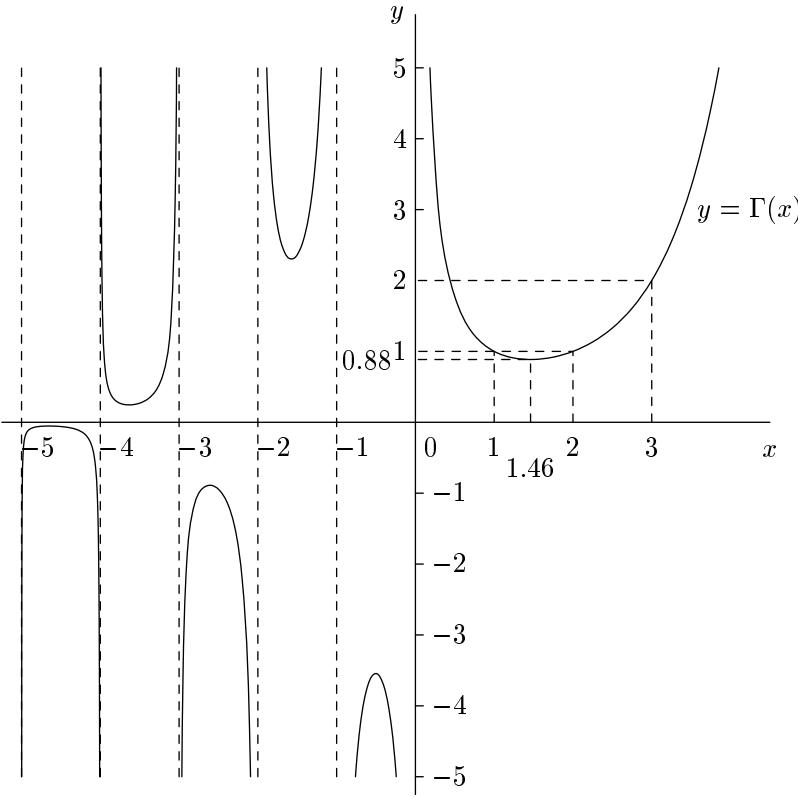
\includegraphics[keepaspectratio]{images/part002_cfbcc1f6.jpg}}\\
Fig. 1\\
and consequently \(\Gamma''(x)\) has the same sign as \(\Gamma(x)\) ; thus \(\Gamma\) is convex for x \textgreater{} 0 and for \(-(2n + 2) < x < -(2n + 1)\) , and concave for \(-(2n + 1) < x - 2n\) ( \(n \in N\) ); one deduces from this that, on the intervals where \(\Gamma\) is convex, \(\Gamma'(x)\) increases from \(-\infty\) to \(+\infty\) , and on the intervals where \(\Gamma\) is concave, \(\Gamma'(x)\) decreases from \(+\infty\) to \(-\infty\) . Whence the graph of \(\Gamma\) (fig.~1).
